\chapter{Experiments \& Results}
\lhead{Chapter 4 \emph{Experiments \& Results}}
\label{chap:4}
%\autoref{cha:4}

\bigskip

In this chapter the results of the revisit time calculation are the first to be presented. Then, several experiments are demonstrated, which follow the logical sequence of a possible application use. Namely, examples of user's requests that ask to find out if there are currently operational satellites that have some specific properties and to name them, are shown. Then, based on the application's answer, the user can opt to find the revisit time of a group of satellites or of a constellation. Thus, several experiments related to the calculation of the collective revisit time are demonstrated.

Additionally, a user has the possibility to find the position of a prospective new satellite, which can achieve together with a group of satellites already in orbit a more frequent revisit time. It also needs to be mentioned that the software calculates the revisit time specified in terms of the latitude. As a default approach the revisit time at the equator is found, however the software can calculate the revisit time at any latitude of interest to the user.

It also needs to be mentioned that for the experiments and results that are presented, 300 orbits has been selected to be the duration of the simulations. Since the average period of the experimented satellites and the EO satellites in LEO that have been plugged in the database (Section \ref{database_ch3}) is approximately 100 minutes, then in 300 orbits, 20 days have elapsed. Based on the revisit rates of satellites with similar characteristics, 20 days is a period in which the revisit time of those satellites can be acquired \cite{Christopherson}. Nevertheless, for satellites, which fall into a different category than of LEO or EO and orbit for example in higher altitudes, this assumption needs to be changed.

\bigskip
\section{Revisit time calculation of single satellites}
\bigskip

As it was mentioned in Chapter \ref{added value}, the creation of a database, which contains information about the orbit and attributes of the on-board sensors of LEO satellites in the field of EO, is of great importance for assessing the added value of a planned EO mission. For this reason, the first results to be presented show the revisit time of satellites, which are hosted in the database. Nevertheless, since the application needs also to be tested (Chapter \ref{chap:5}), the results of renowned and well documented satellites, like the Sentinels were chosen to be presented.

The first example to be showed is the satellite Sentinel-2A. In the Figure \ref{revisit_time_Sentinel2A} the average revisit time per longitude cell along the equator can be found. The length of the longitude cell was determined based on the swath width of the satellite's sensor (Equation \ref{grid_interval}), which in this case is 290 km \footnote{\label{Sentinel-2}\textit{Available at: https://sentinel.esa.int/web/sentinel/missions/sentinel-2 (Accessed November 20, 2020)}}. As it can also be seen in the figure, there are some longitude cells which the satellite does not pass. After having computed the average revisit time per longitude cell, the average revisit time at equator is found, which is depicted in blue line in the figure. As shown, the average revisit time at equator of Sentinel-2A is around 10 days (Figure \ref{revisit_time_Sentinel2A}).

\begin{figure}
\centering
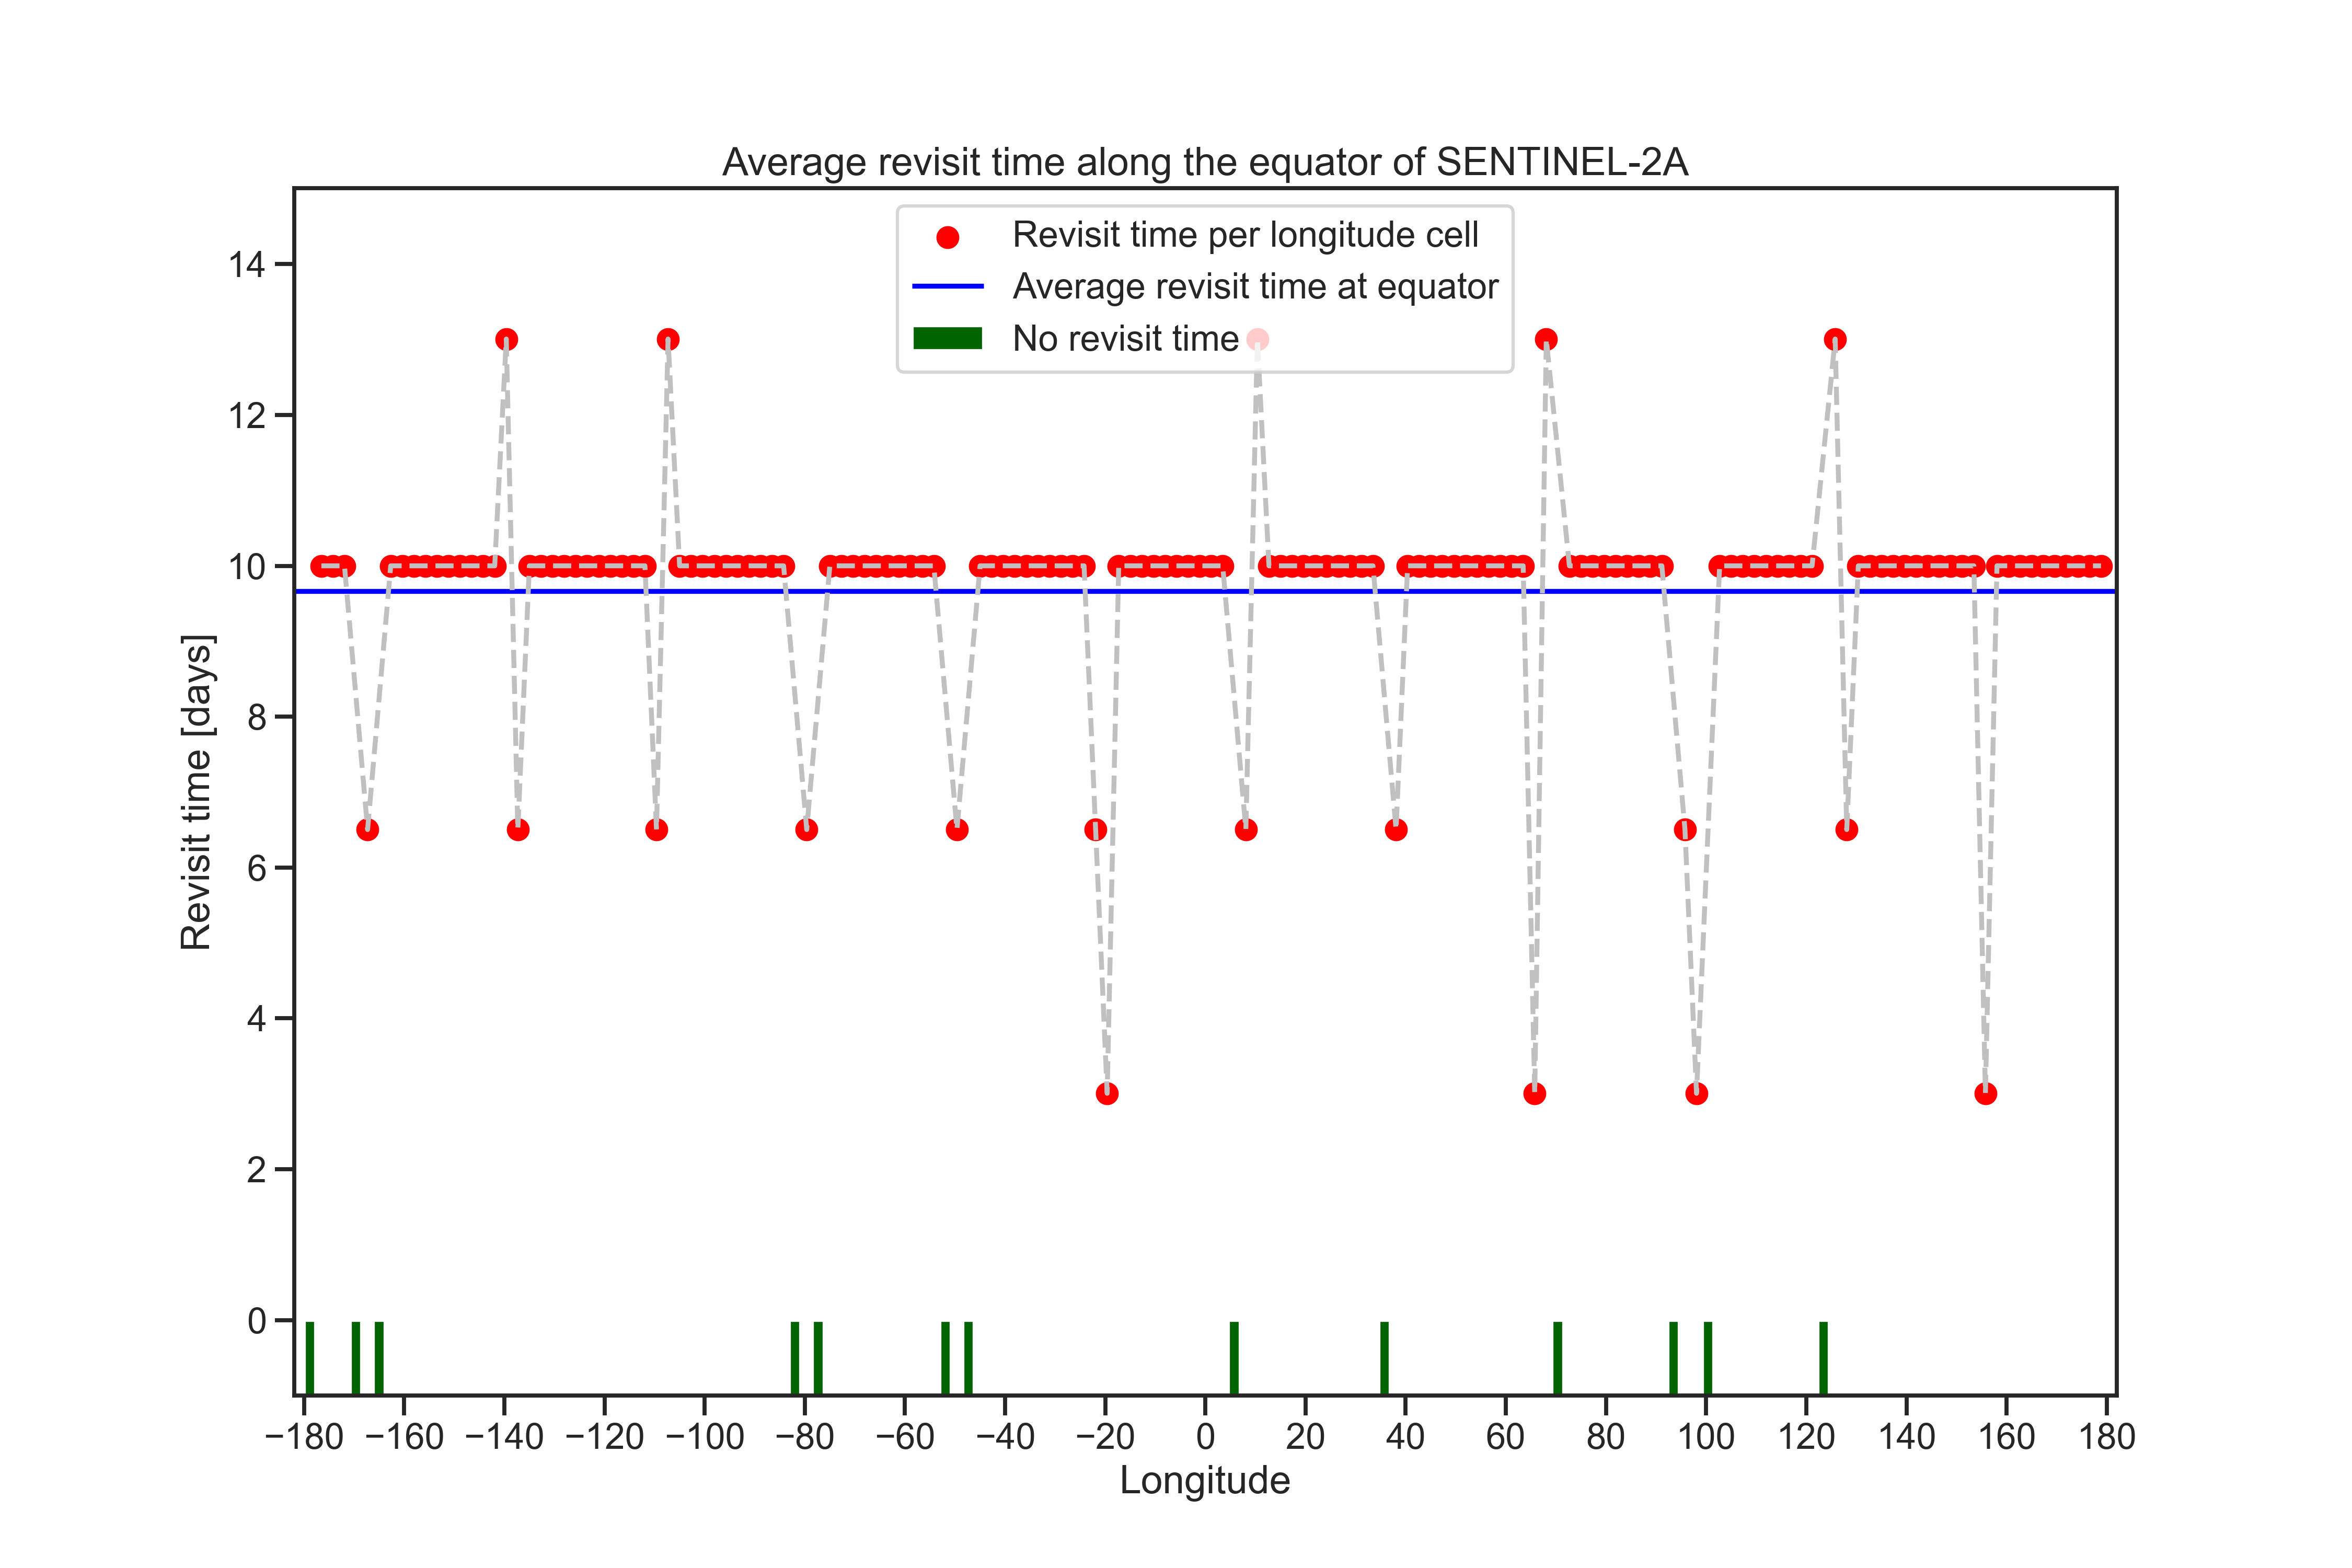
\includegraphics[width=0.9\textwidth]{Images/revisit_time_of_SENTINEL-2A.png}\caption{Average revisit time per longitude cell along the equator. The length of the longitude cell was determined based on the swath width of the satellite's sensor (Equation \ref{grid_interval}). The average revisit time at the equator of Sentinel-2A is 9.66 days.}
\label{revisit_time_Sentinel2A}
\end{figure}
% Run the code main_code_db_aggregated.py

An equivalent graph showing the average revisit time at equator of Sentinel 3A \footnote{\label{Sentinel3A_source}\textit{Available at: https://sentinel.esa.int/web/sentinel/user-guides/sentinel-3-synergy/coverage (Accessed November 20, 2020)}} can be found in Figure \ref{revisit_time_Sentinel3A}. The average revisit time at the equator for this satellite is less than 2 days, since the swath width of its optical instrument is as large as 1250 km. For validation purposes, two other graphs showing the average revisit time of satellites are presented. In the Figure \ref{revisit_time_of_ALSAT 1B}, the revisit time of the Algerian Alsat-1B satellite can be found, whereas in Figure \ref{revisit_time_of_GOMX-4A} the one of the Danish GOMX-4A satellite \cite{Christopherson}.

\begin{figure}
\centering
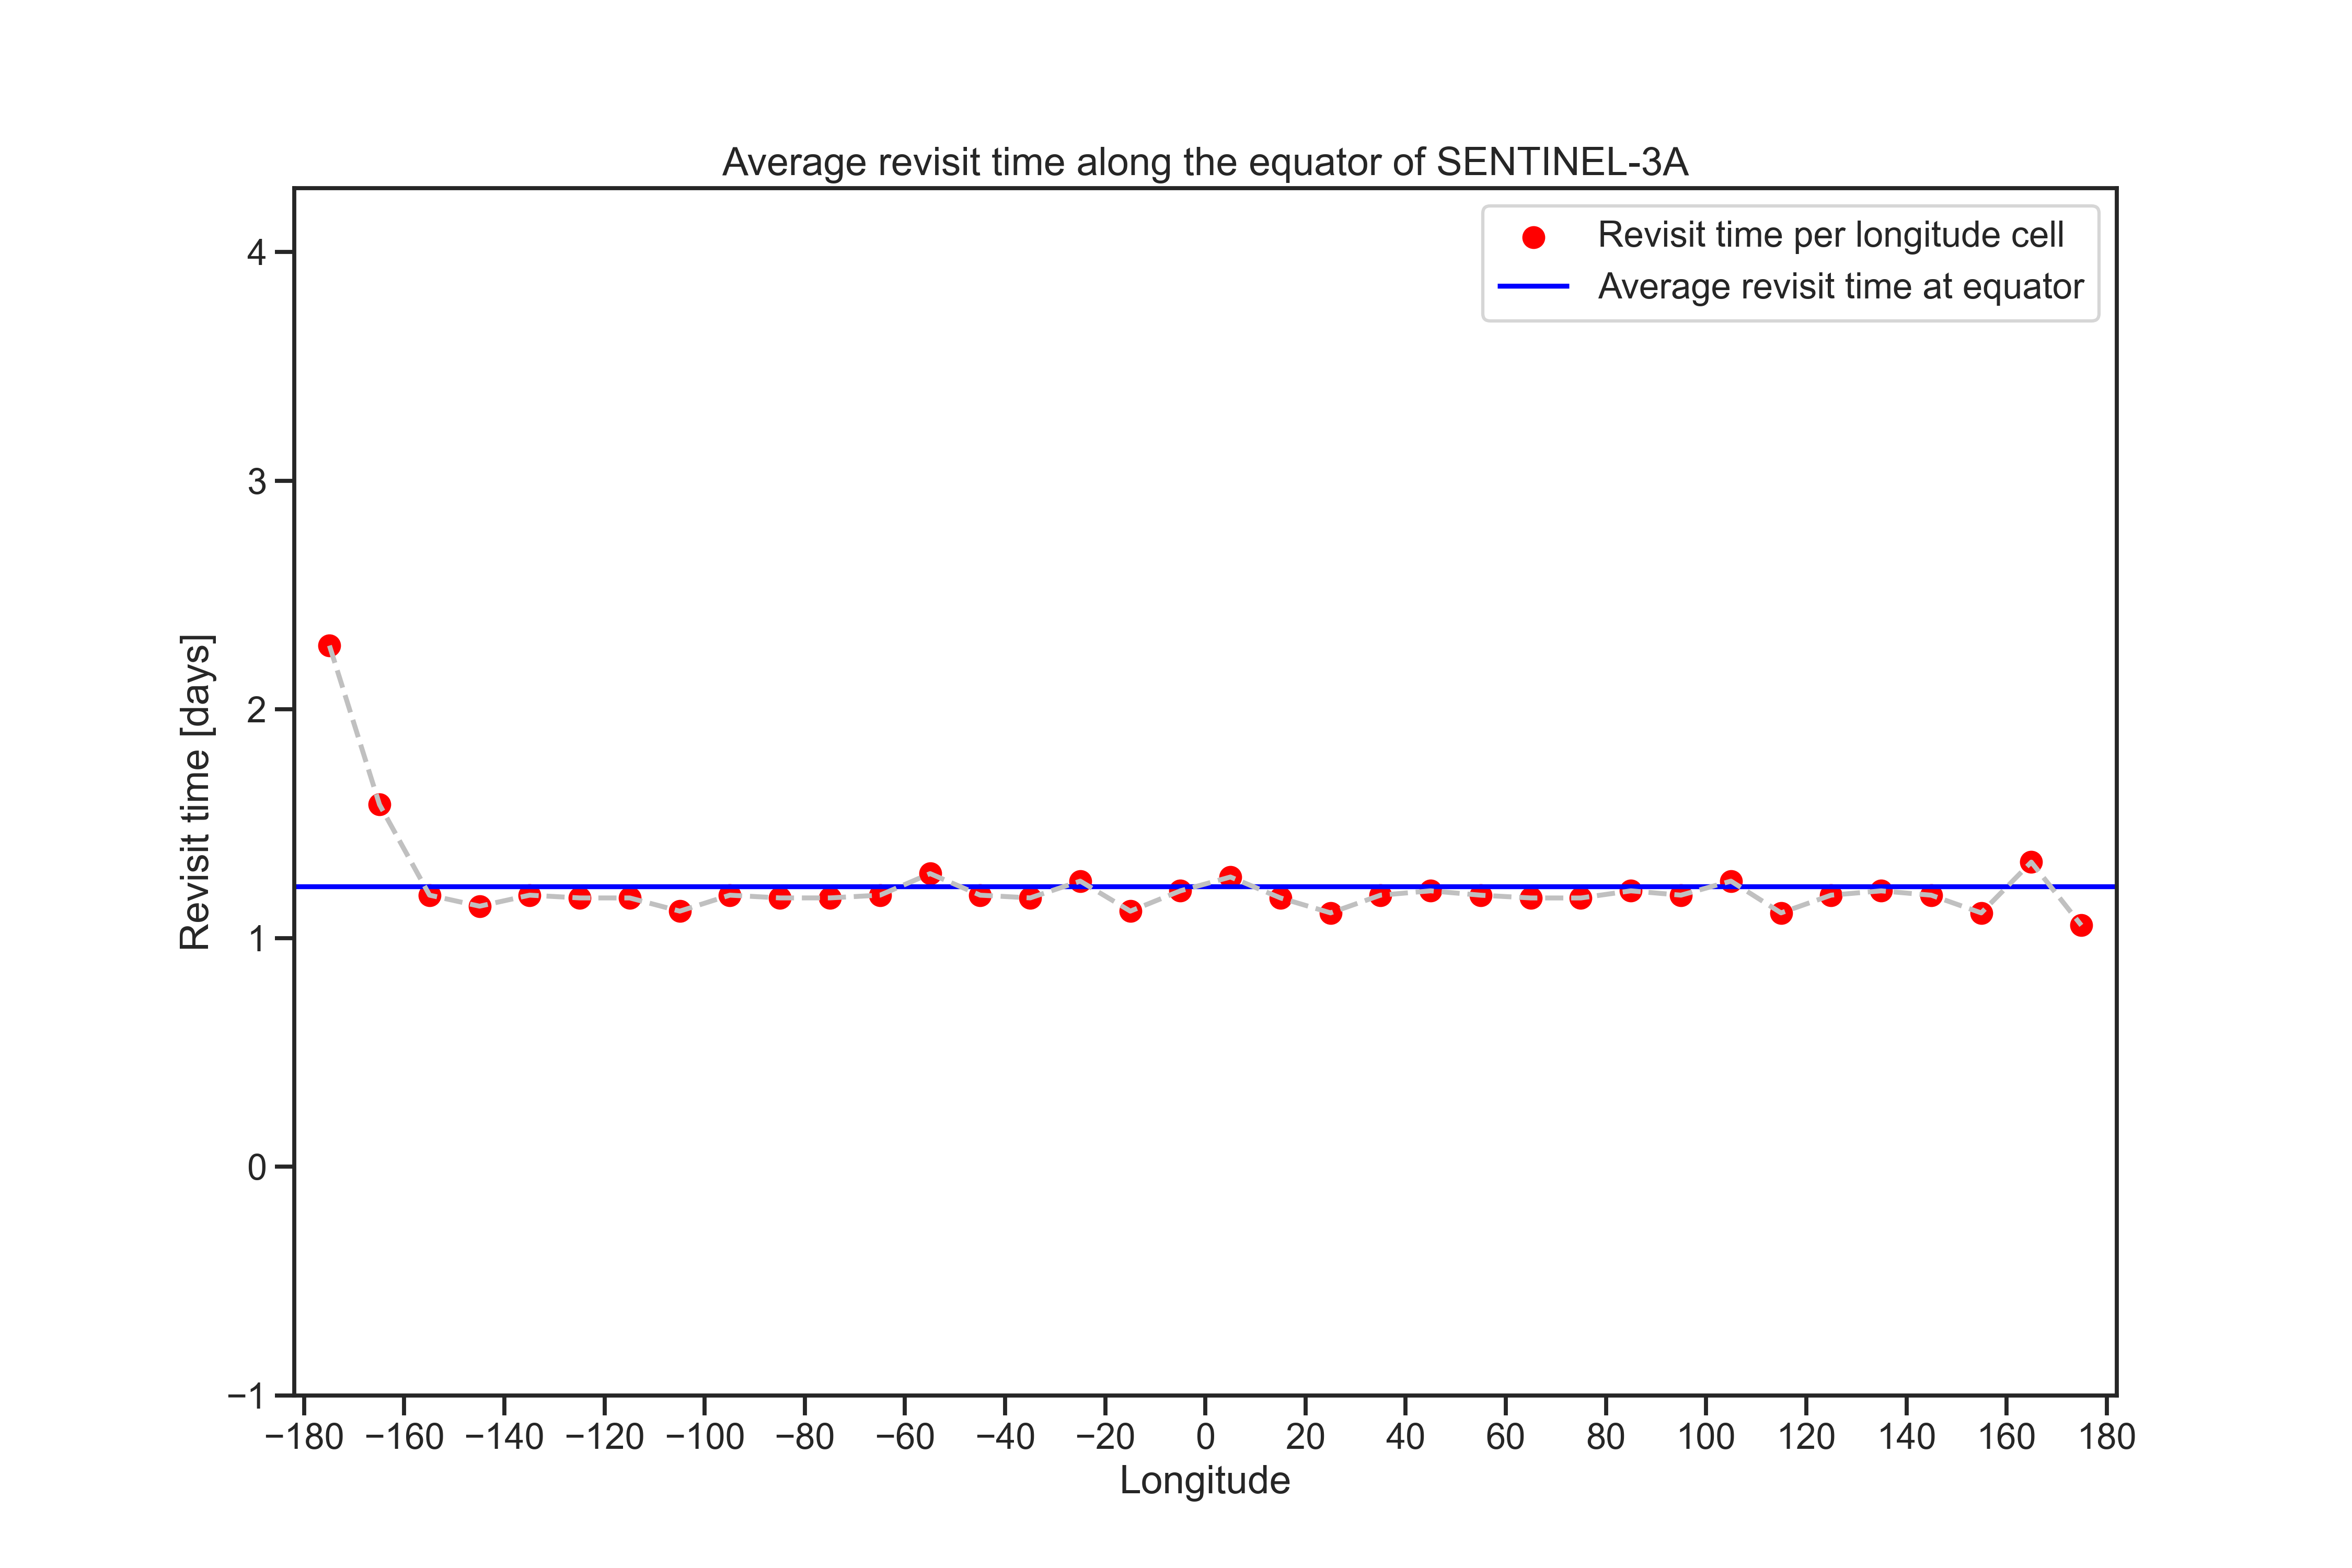
\includegraphics[width=0.9\textwidth]{Images/revisit_time_of_SENTINEL-3A.png}\caption{Average revisit time per longitude cell along the equator. The average revisit time at the equator of Sentinel-3A is 1.22 days.}
\label{revisit_time_Sentinel3A}
\end{figure}
% Run the code main_code_db_aggregated.py

\begin{figure}
\centering
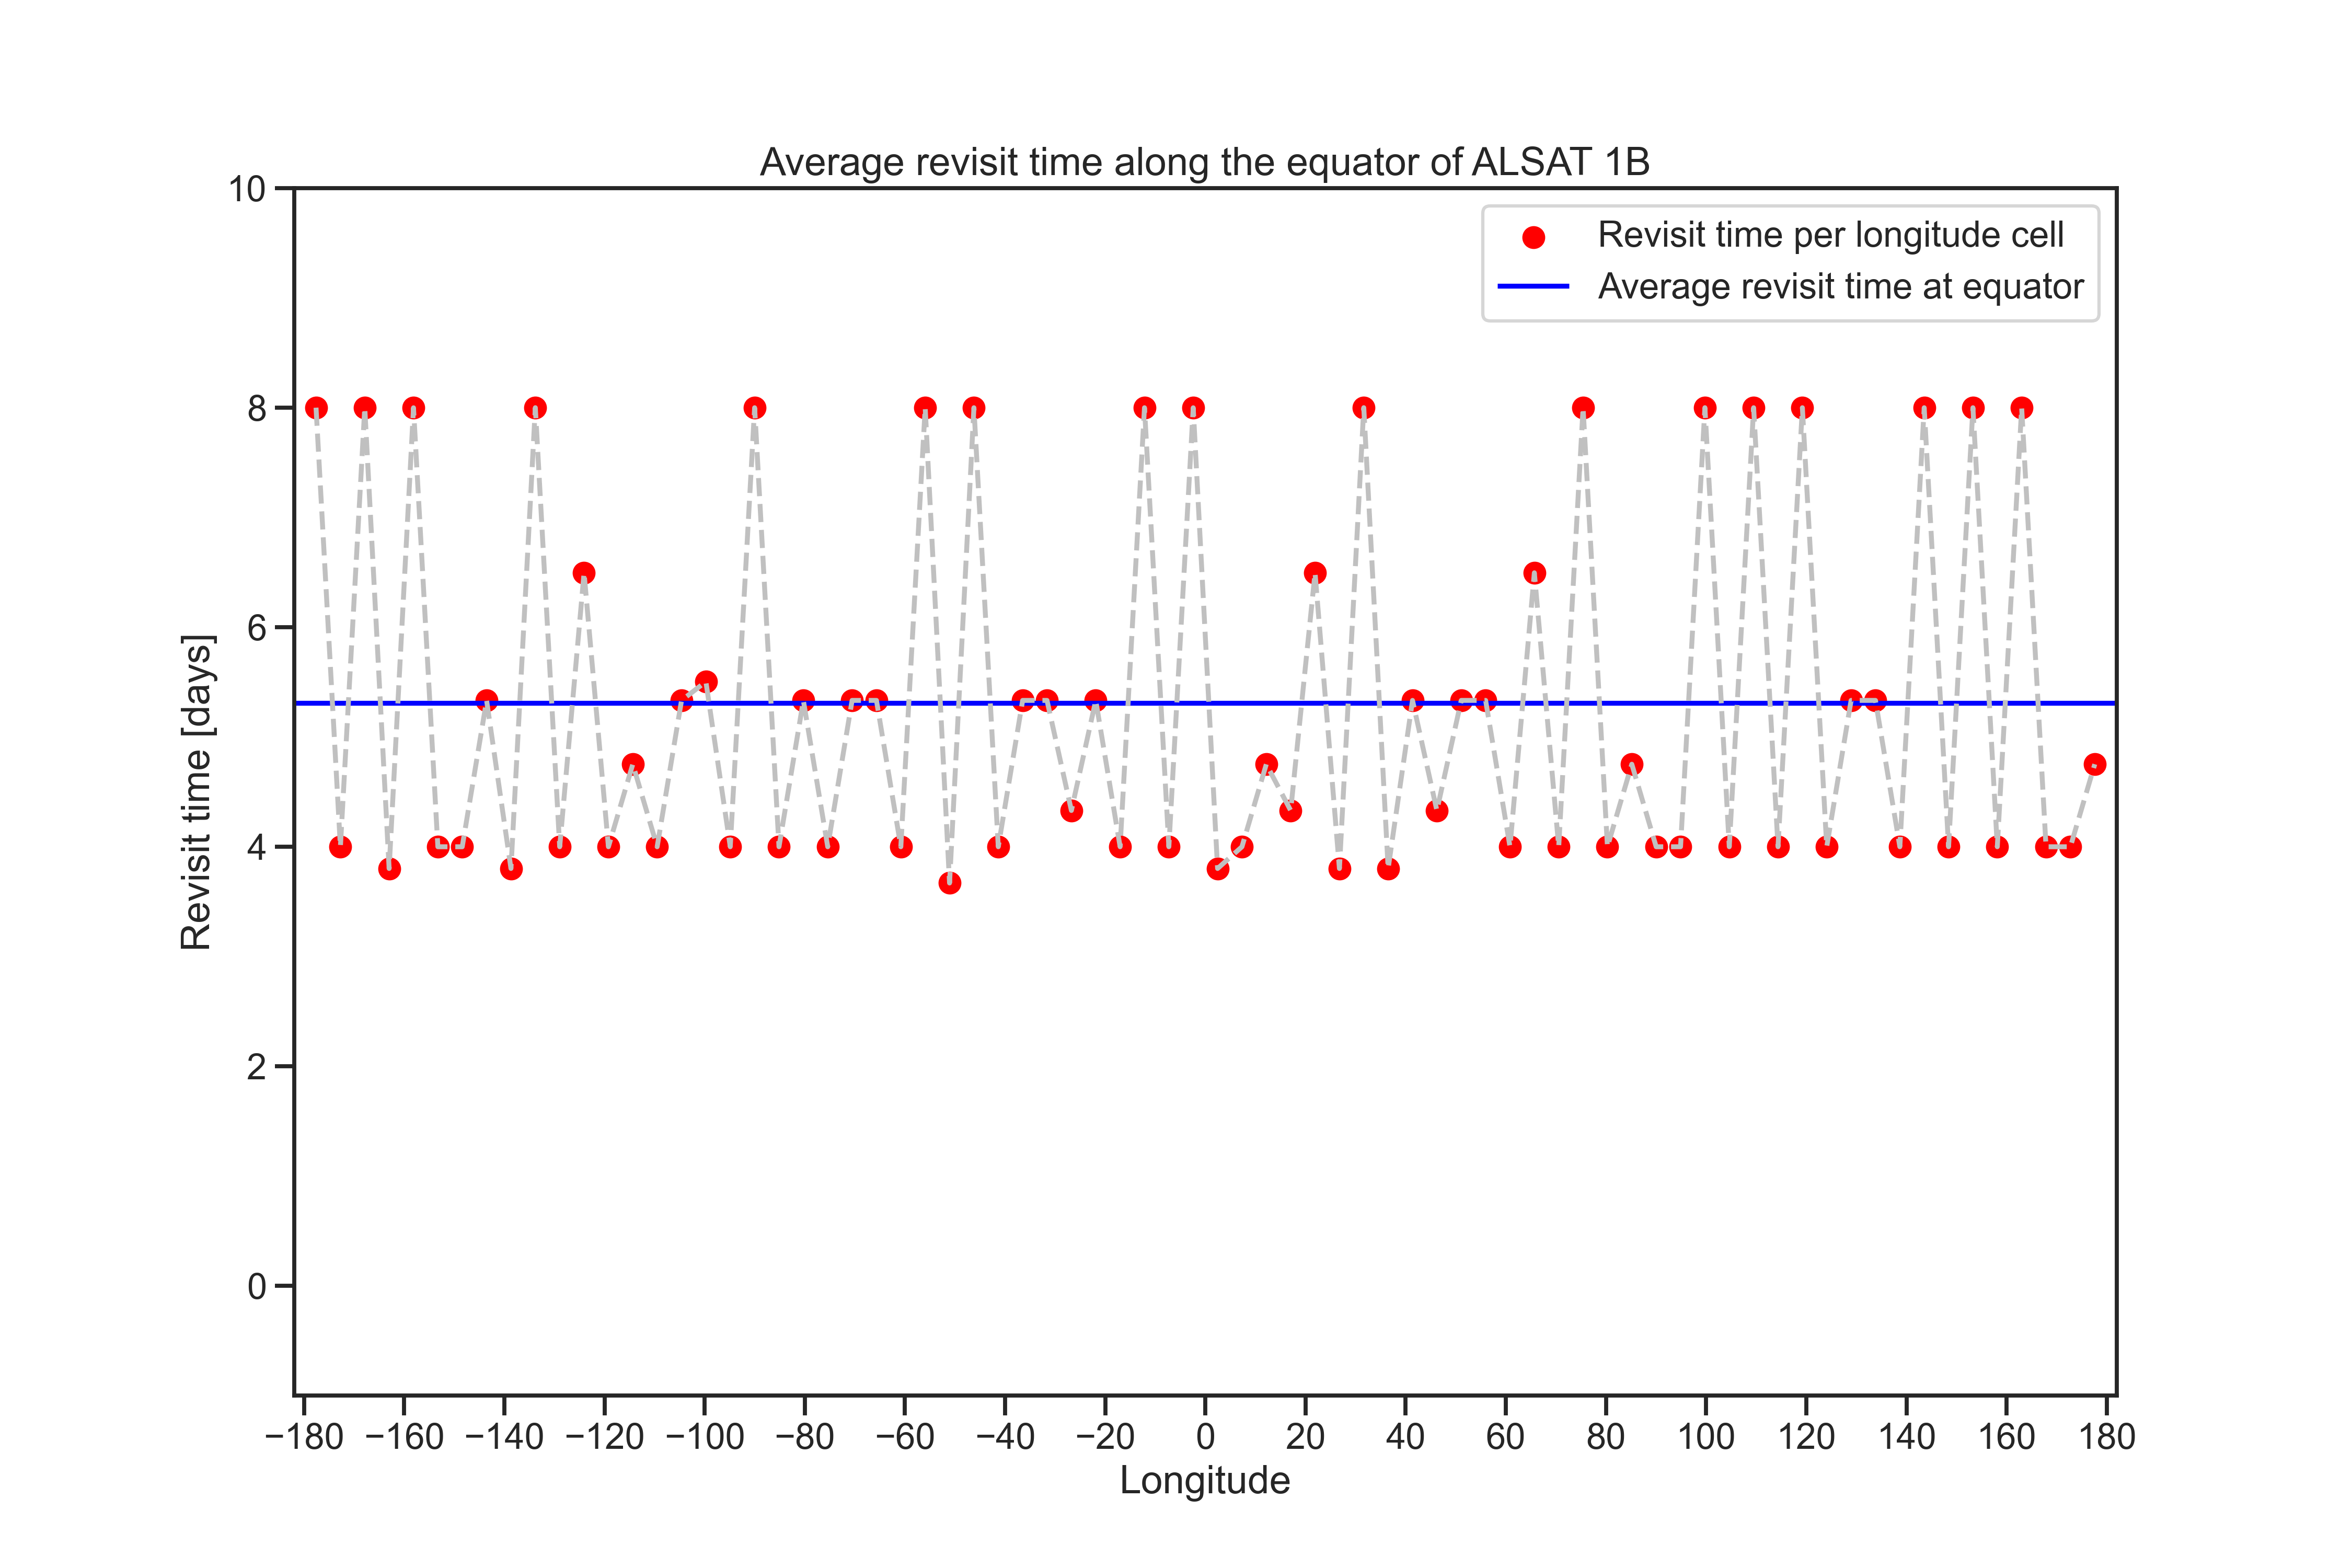
\includegraphics[width=0.9\textwidth]{Images/revisit_time_of_ALSAT_1B.png}\caption{Average revisit time per longitude cell along the equator. The length of the longitude cell was determined based on the swath width of the satellite's sensor (Equation \ref{grid_interval}). The average revisit time at the equator of Alsat-1B is 5.31 days.}
\label{revisit_time_of_ALSAT 1B}
\end{figure}
% Run the code main_code_db_aggregated.py

\begin{figure}
\centering
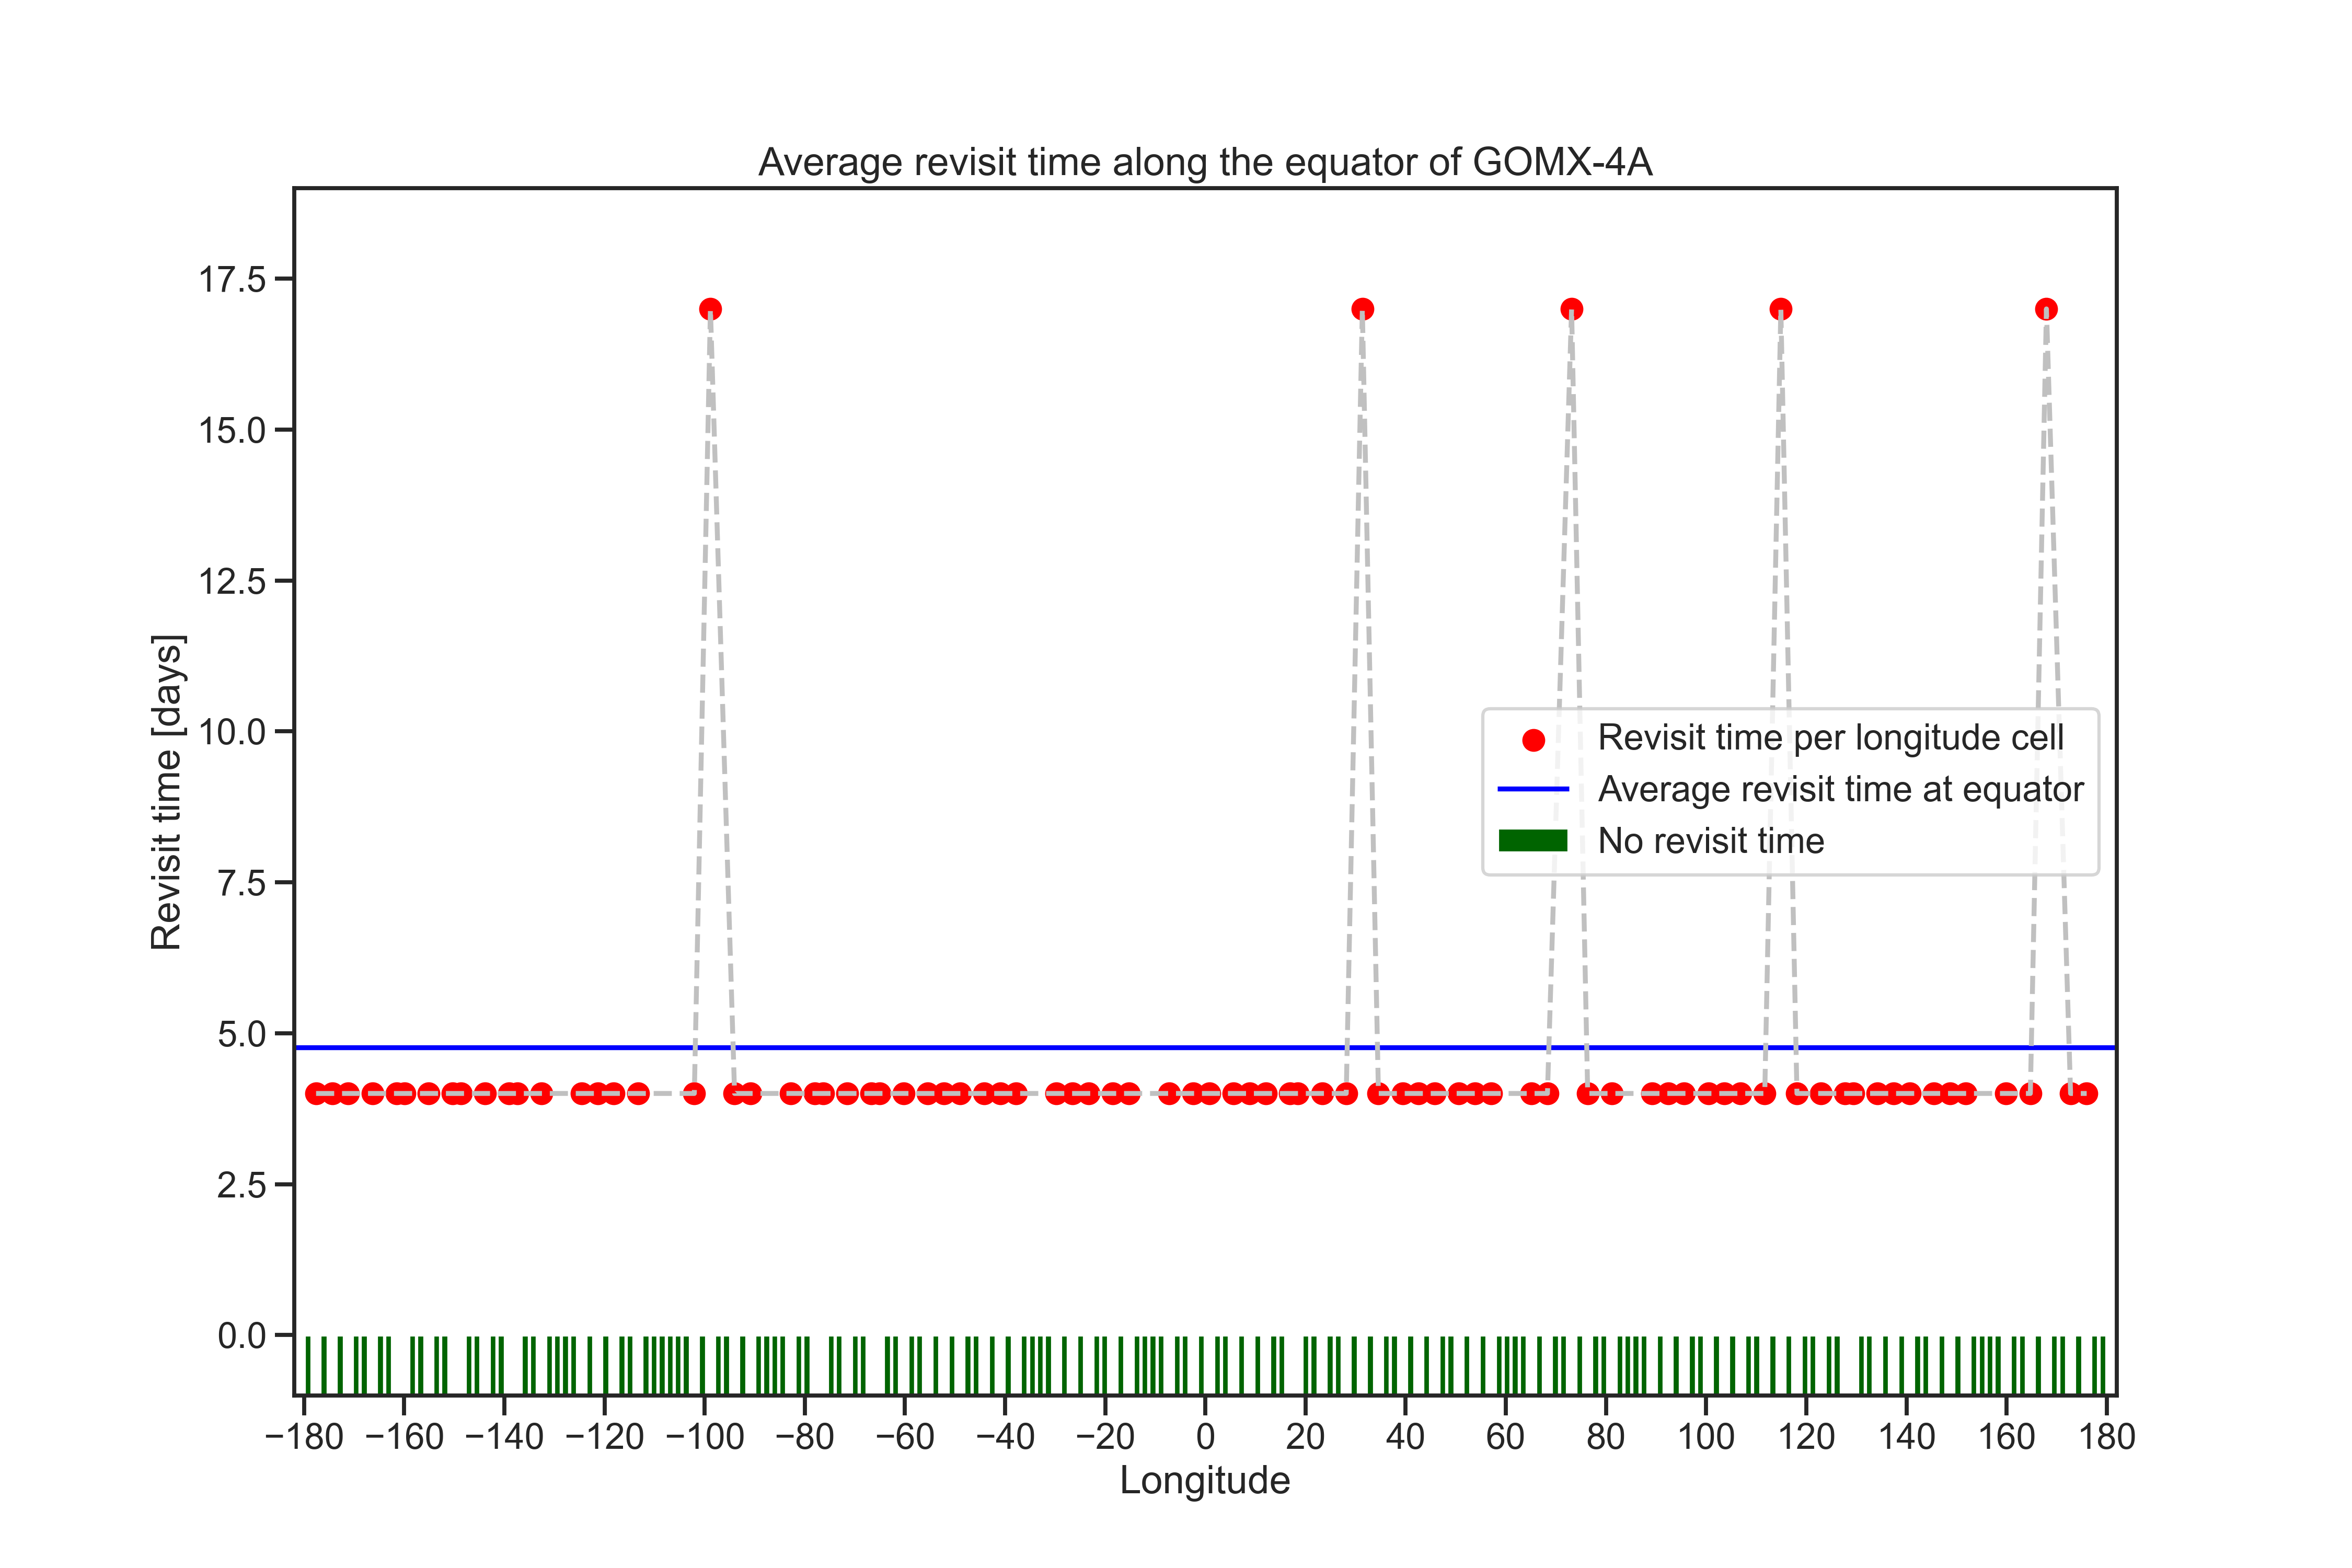
\includegraphics[width=0.9\textwidth]{Images/revisit_time_of_GOMX-4A.png}
\caption{Average revisit time per longitude cell along the equator. The average revisit time at the equator of GOMX-4A is 4.77 days.}
\label{revisit_time_of_GOMX-4A}
\end{figure}
% Run the code main_code_db_aggregated.py

\bigskip
\section{Request to find operational satellites with certain \\properties}
\bigskip

Another capability that this application brings is that the user can request to find whether there are currently operational satellites, which have certain characteristics or offer specific properties that are of the user's interest. The properties that a user can specify, are related to the various fields of attributes that were added to the database.

To be more exact, these properties can pertain to the date that a satellite was launched, its operational lifetime, the type of sensors that it has on board, and the resolution that they can achieve, as well as the type and the objective of the mission, such as whether it is a commercial, civil, or defense mission and the main goal and focus of the mission (Figure \ref{classification_1st_layer}, \ref{classification_2nd_layer}). All the above information about the satellites, which have been added to the database, can be found in the tables \ref{table:1}, \ref{table:2}, \ref{table:3} in the section of Appendix. Moreover, the user can find out whether a satellite, which has a specific desirable revisit time at the equator exists. This information of the revisit time has been added to the database after calculating it for all the elements of the database based on the procedure that was described in Chapter \ref{chap:3}.

\bigskip

The first experiment to be presented is of a user, who wants to find which are the satellites that have an active sensor, have less than six days of revisit time at the equator and have more than three years of operational lifetime. In the algorithm \ref{Request1}, the whole procedure can be found, together with the output that the code produced. As a second experiment, a user wants to find which are the satellites that have as their main objective the monitor of the land ("Land monitoring") and the resolution of their sensors is four meters (Algorithm \ref{Request2}).

\begin{algorithm}[H] % When you have [H], then the algorithm appears exactly under the text. If you don't write it then, it goes at the end of the whole pdf.
\caption{Request regarding sensor type, revisit time \& operational lifetime.}\label{Request1}
\hspace*{\algorithmicindent} \textbf{Input: }\\
\hspace*{\algorithmicindent} $\textcolor{purple}{sensor } \gets \text{'active'}$ \\
\hspace*{\algorithmicindent} $\textcolor{purple}{days } \gets \text{6}$ \\
\hspace*{\algorithmicindent} $\textcolor{purple}{lifetime } \gets \text{'3 years'}$
\begin{algorithmic}[1]
\Procedure{}{}
\State $\text{Connection to the database}$ 
\State $\textbf{SELECT } \textit{name }$ \Comment{The output will be the name of the satellites}
\State $\textbf{FROM } \textit{attributes }$ \Comment{\textit{attributes}: main table of the database}
\State $ \textbf{WHERE:} $
\State \hspace*{\algorithmicindent} $\textit{type_of_sensor = } \text{ } \textcolor{purple}{sensor} \textbf{ AND} $
\State \hspace*{\algorithmicindent} $\textit{revisit_time < } \text{ } \textcolor{purple}{days} \textbf{ AND}$
\State \hspace*{\algorithmicindent} $\textit{(now() - } \textbf{CAST}\textit{(date_launched } \textbf{AS TIMESTAMP) <  } \text{ } \textcolor{purple}{lifetime} \text{ ;}$
\EndProcedure
\Comment{\textit{now()}: function showing current date}
\end{algorithmic}
\hspace*{\algorithmicindent} \textbf{Output:}\\ \hspace*{\algorithmicindent} \textit{[Sentinel-3B, Sentinel-6, SAOCOM-1A, NOVASAR-1, RCM-1, RCM-2, RCM-3]}
\end{algorithm}

\begin{algorithm}[H] % When you have [H], then the algorithm appears exactly under the text. If you don't write it then, it goes at the end of the whole pdf.
\caption{Request regarding mission objective \& sensor resolution.}\label{Request2}
\hspace*{\algorithmicindent} \textbf{Input: }\\
\hspace*{\algorithmicindent} $\textcolor{purple}{objective } \gets \text{'land monitoring'}$ \\
\hspace*{\algorithmicindent} $\textcolor{purple}{meters } \gets \text{4}$
\begin{algorithmic}[1]
\Procedure{}{}
\State $\text{Connection to the database}$ 
\State $\textbf{SELECT } \textit{attributes.name, attributes.id }$ \Comment{The output will be the name of the satellites and their unique database ID}
\State $\textbf{FROM } \textit{attributes }$ \Comment{\textit{attributes}: main table of the database}
\State $ \textbf{INNER JOIN } \textit{classification }$ Comment{\textit{classification}: table with information about type and mission objectives}
\State $ \textbf{ON } \textit{classification.environmental_monitoring = environmental_monitoring} $
\State $ \textbf{WHERE:} $
\State \hspace*{\algorithmicindent} $\textit{environmental_monitoring = } \text{ } \textcolor{purple}{objective} \textbf{ AND} $
\State \hspace*{\algorithmicindent} $\textit{resolution = } \text{ } \textcolor{purple}{meters}$
\EndProcedure
\end{algorithmic}
\hspace*{\algorithmicindent} \textbf{Output:}\\ \hspace*{\algorithmicindent} \textit{[NOVASAR-1, CARTOSAT-3, HUANJING-2B, HUANJING-2A, JILIN-01 GAOFEN-3J, ... (9 more JILIN-01 GAOFEN satellites), SENTINEL-1B, SENTINEL-1A]}
\end{algorithm}

% Change the Algorithm2 with "resolution" to have AT LEAST this number <=. So, first create the range in the column of resultion (in the database probably). Check-google operators like: "BETWEEN" or "LIKE" or "substring_index()" --> [SQL search interger range from number with dash] or [range in sql with hyphen]. It is not in the scope of this thesis, to solve such a problem, however I have investigated that there is a way to do it - Check: https://stackoverflow.com/questions/45054978/mysql-search-integer-range-from-number-with-dash

From the second experiment, the user found that there are 16 satellites that have the desired properties, which can be also seen in the section of the \textit{Output} in the algorithm \ref{Request2}. An extension of this request is that the user wants to know the revisit time of a specific latitude from those satellites. For this example, the latitude of 48$^{\circ}$ was selected, which is the latitude of Munich. Therefore, by inserting into the software the ID of those satellites that were just found and the 48$^{\circ}$ latitude, the revisit time at this latitude is calculated for all 16 satellites. In the Figure \ref{revisit_time_at_latitude_48}, it can be seen that NOVASAR-1 is the satellite, which has the most frequent revisiting rate at Munich's latitude, which is less than 2 days.

\begin{figure}
\centering
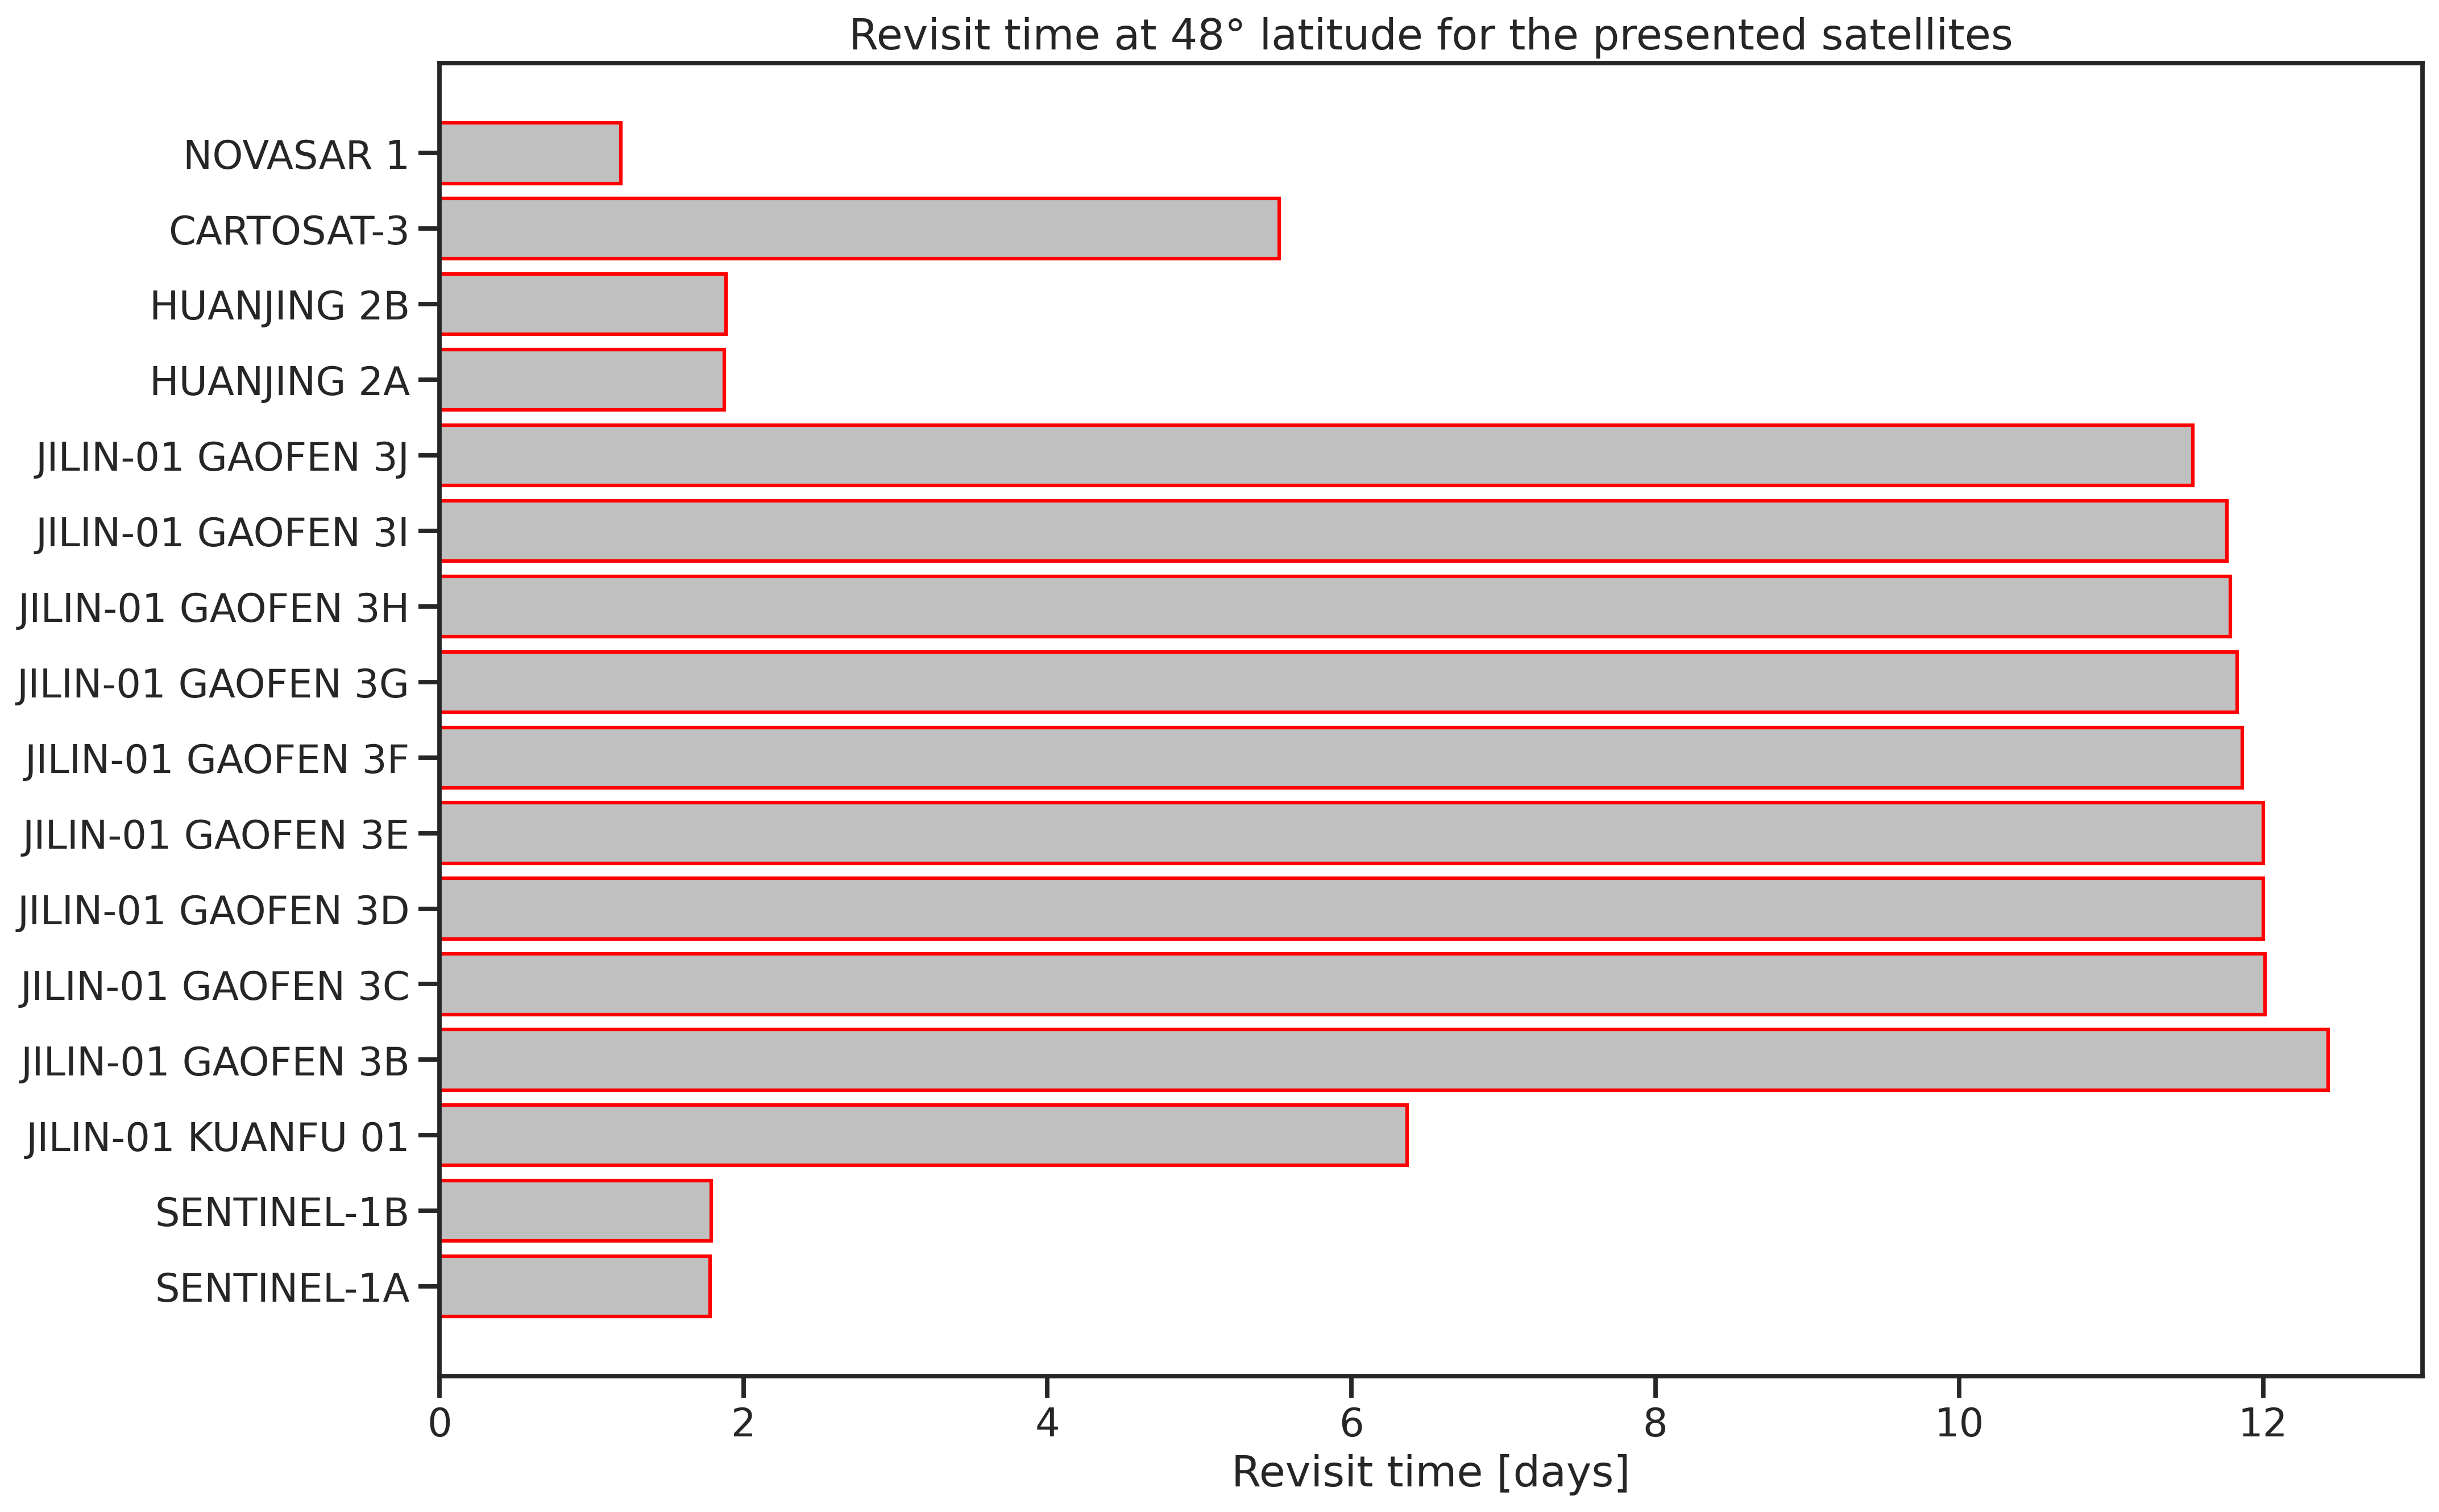
\includegraphics[width=0.9\textwidth]{Images/revisit_time_at_latitude_48.png}
\caption{The revisit time at 48$^{\circ}$ latitude for a group of satellites, which group was found from a user's request (Algorithm \ref{Request2}).}
\label{revisit_time_at_latitude_48}
\end{figure}
%First find the id_list from the user.py. Then, for a different latitude and to find which satellite has the minimum revisit time use: main_code_db_latitude.py.

\bigskip
\section{Revisit time calculation of group of satellites/ \\constellation}
\bigskip

The revisit time calculation of a group of satellites or of a constellation is an additional capability of the software. A step in the procedure, which needs attention is the calculation of the mean anomaly of every satellite for the beginning of the simulation. This should be based on the same epoch. Since the TLE set that is stored for every satellite in the database is referred to a specific and probably different epoch than the rest of the satellites, a common epoch, which will serve as the starting point in time for all those satellites is needed.

Before presenting the results of a calculation of the revisit time of a satellite group, the groundtrack of the Sentinel-2A and Sentinel-2B for one orbit is shown, when their simulation starts at the same epoch. These two figures (\ref{groundtrack_Sentinel-2A}, \ref{groundtrack_Sentinel-2B}) are presented in order to be validated in Chapter \ref{chap:5}. 

\begin{figure}
\centering
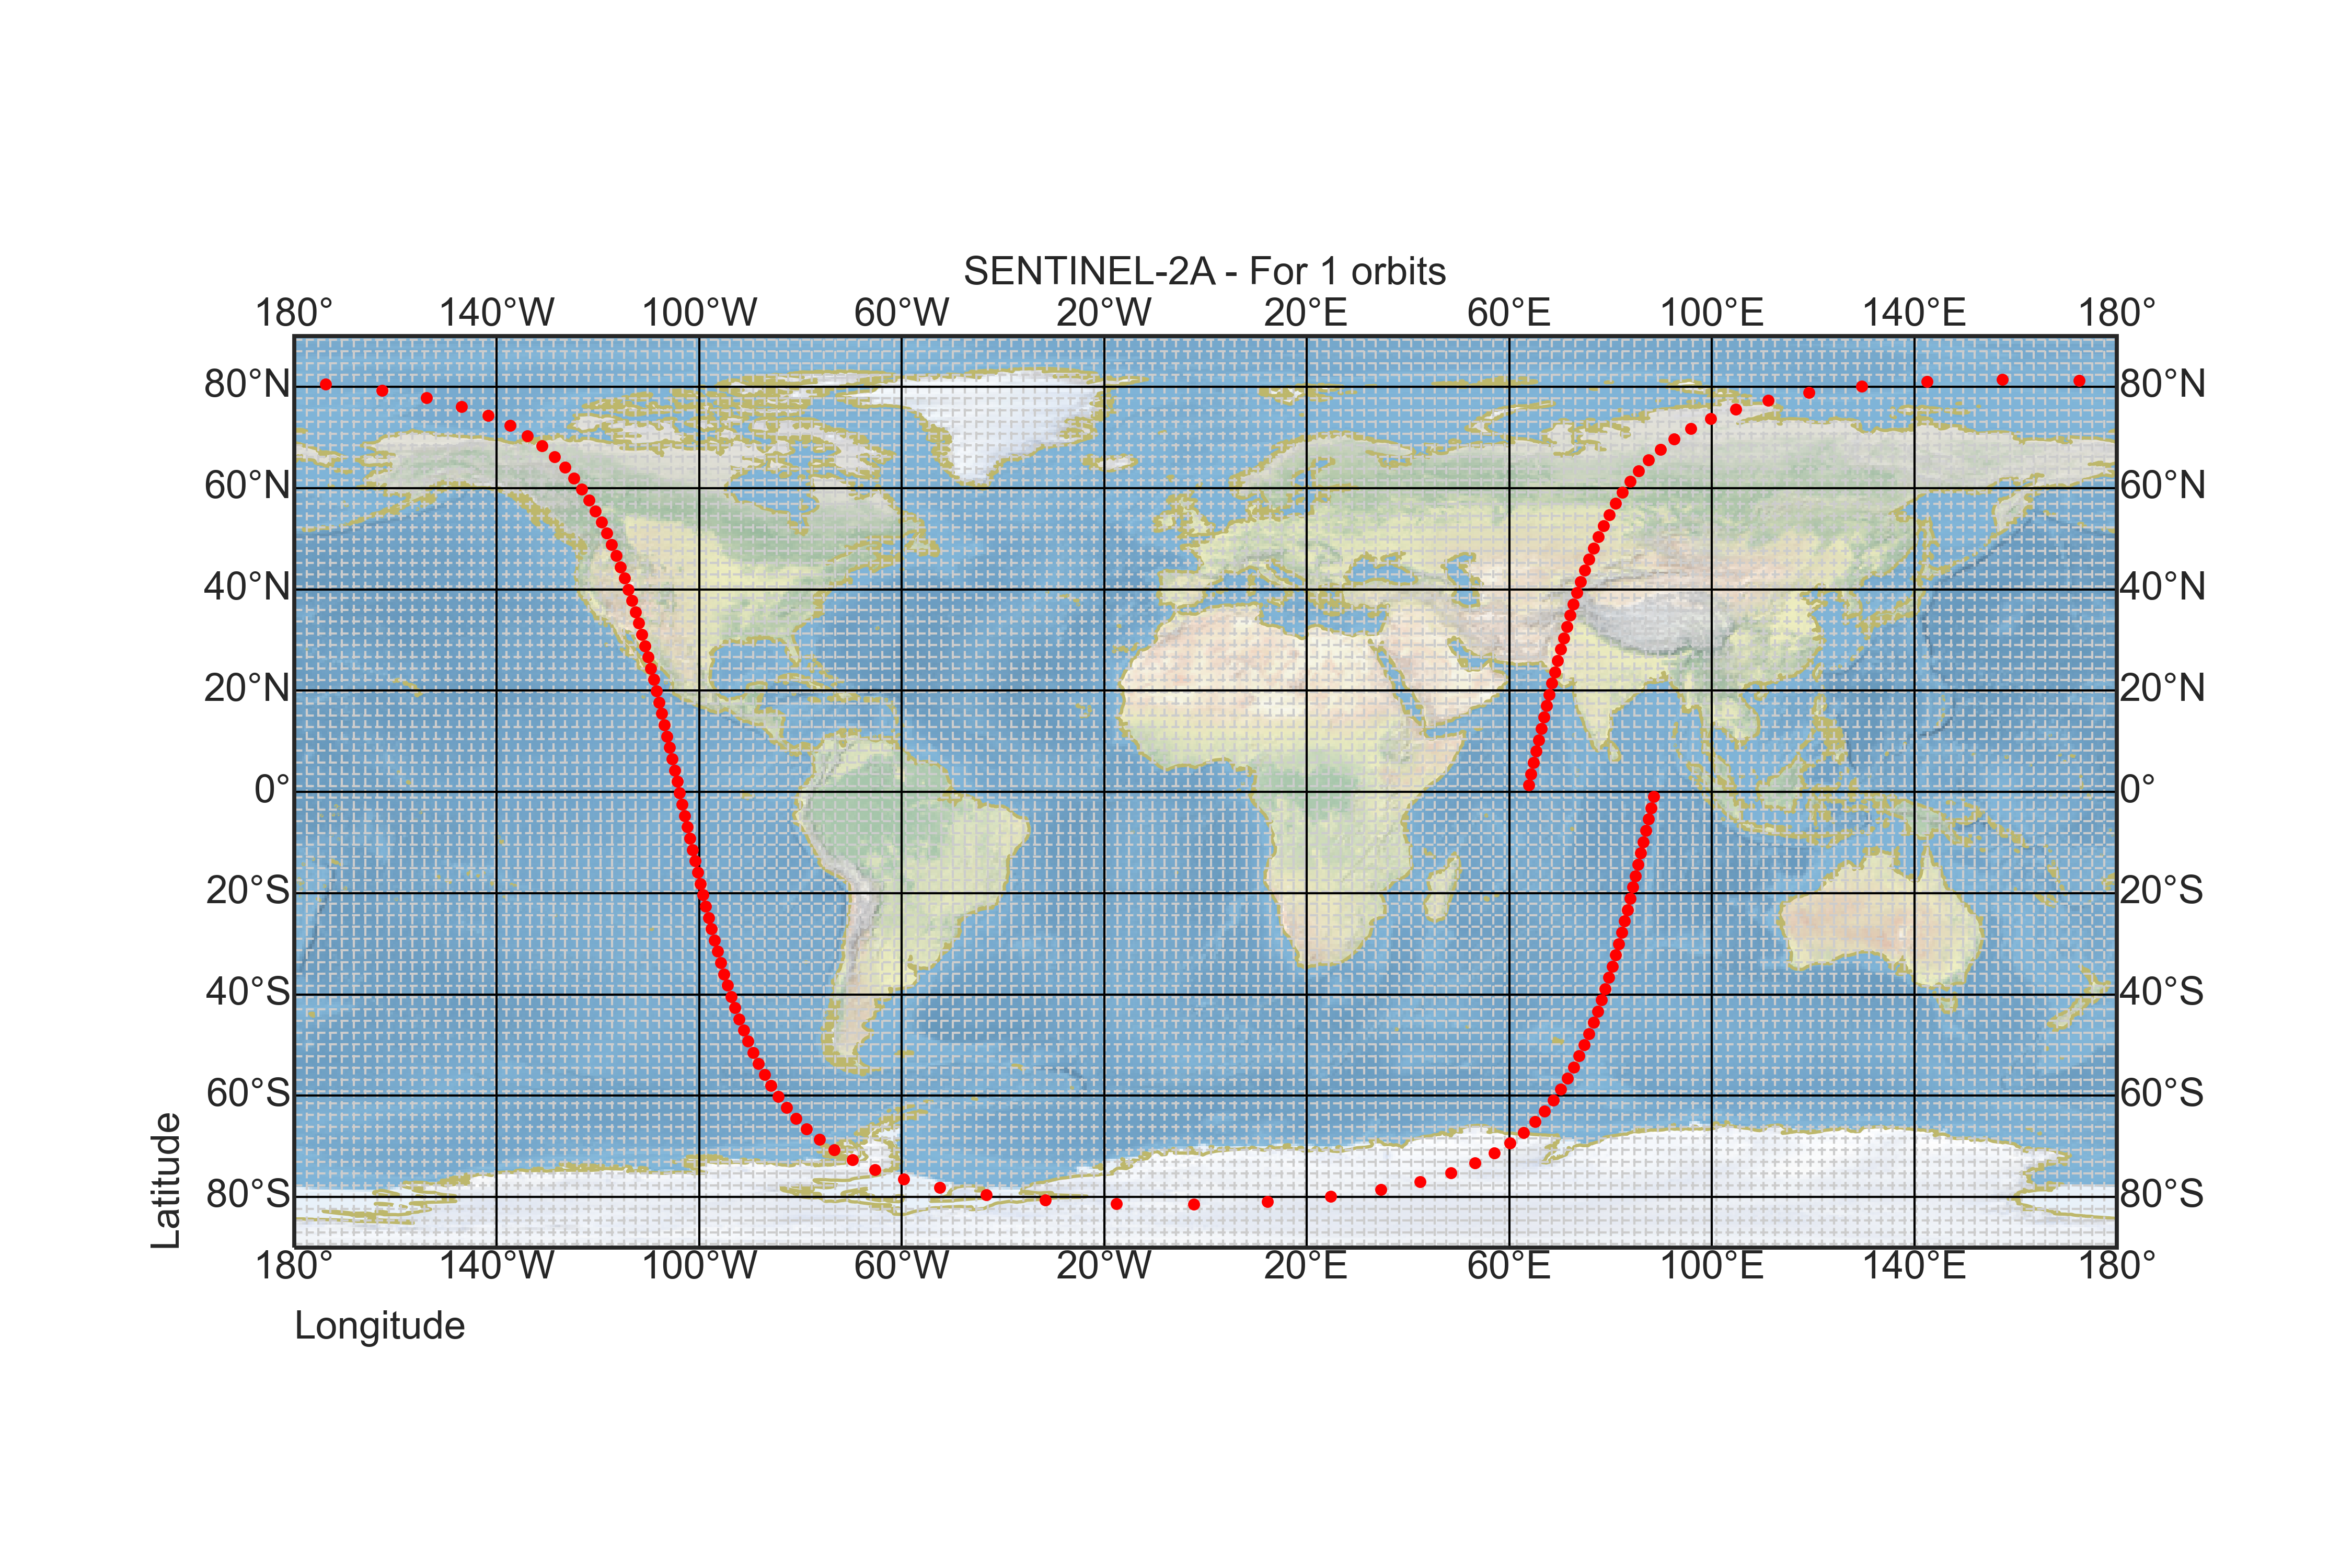
\includegraphics[width=0.9\textwidth]{Images/groundtrack_Sentinel-2A.png}
\caption{The groundtrack of Sentinel-2A for one orbit. The starting point of the satellite's simulation is on the 28th of November 2020 at 00:00}
\label{groundtrack_Sentinel-2A}
\end{figure}

\begin{figure}
\centering
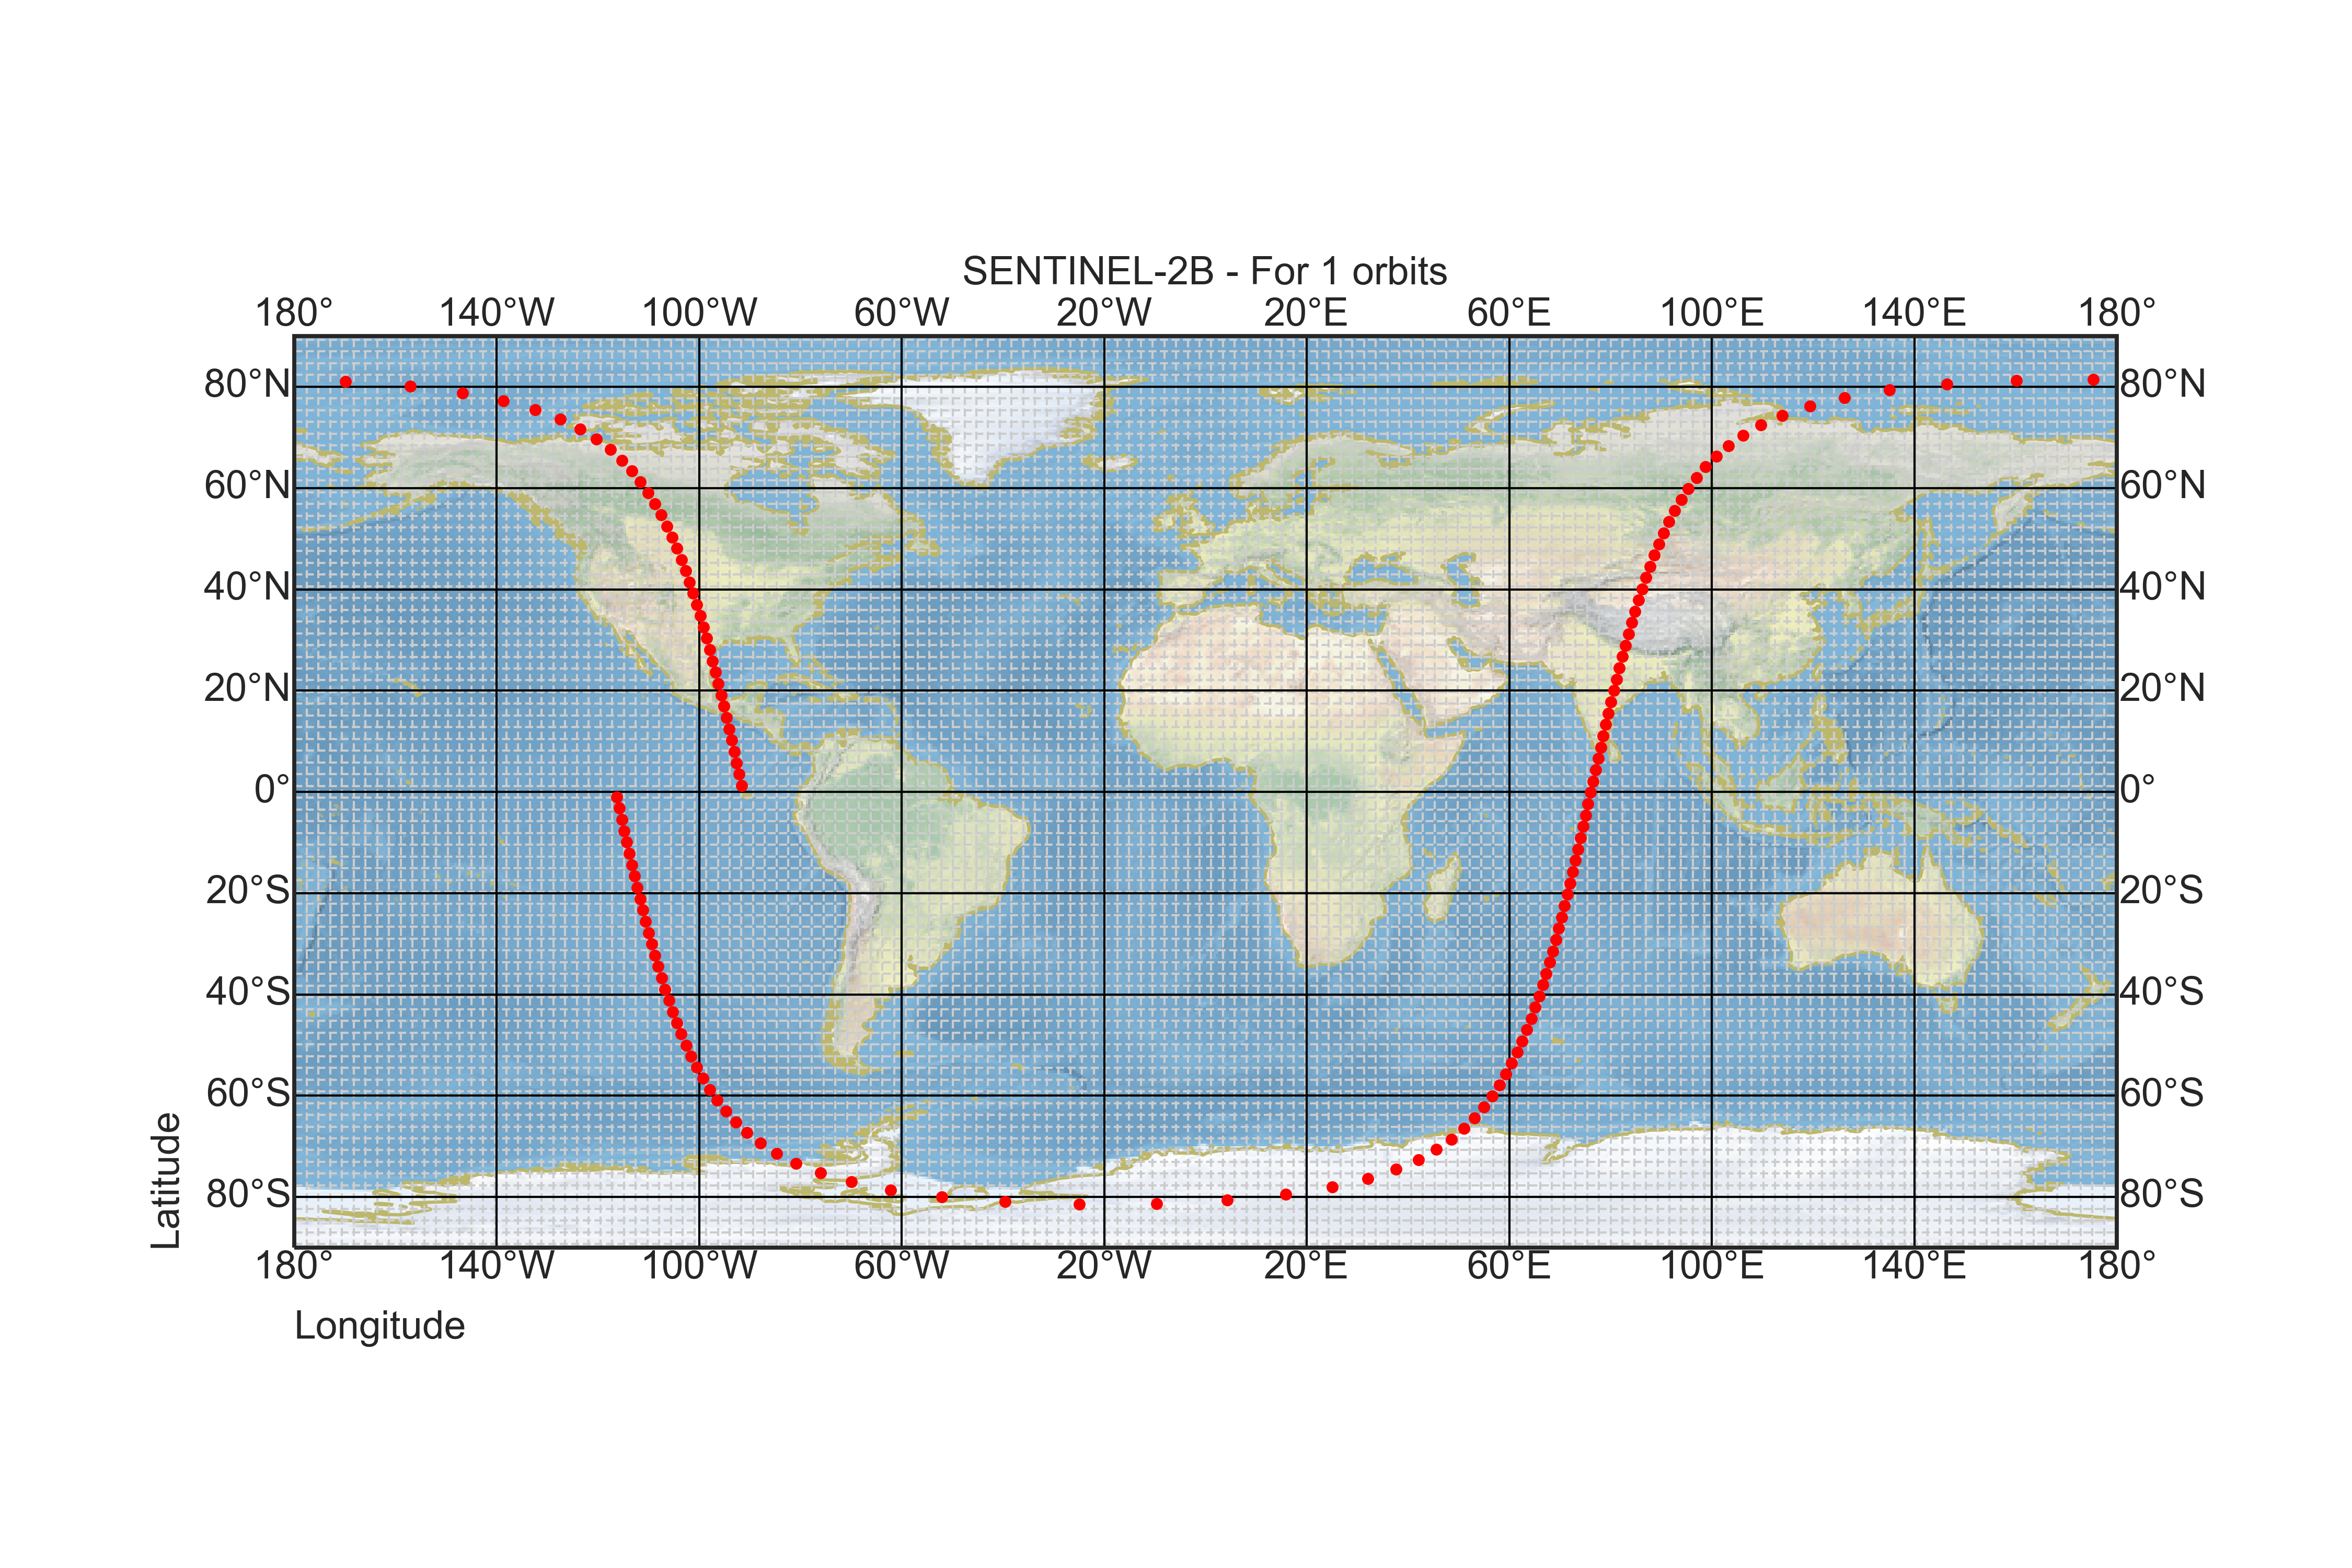
\includegraphics[width=0.9\textwidth]{Images/groundtrack_Sentinel-2B.png}
\caption{The groundtrack of Sentinel-2B for one orbit. The starting point of the satellite's simulation is on the 28th of November 2020 at 00:00.}
\label{groundtrack_Sentinel-2B}
\end{figure}

% Code: main_code_db_aggregated.py

\bigskip
The revisit time calculation of the Sentinel-2 constellation is presented in Figure \ref{revisit_time_of_SENTINEL-2A_SENTINEL-2B}. The average revisit time at the equator is around 5 days. Moreover, the revisit time calculation of the Sentinel-1 constellation was also computed. As shown in Figure \ref{revisit_time_of_SENTINEL-1A_SENTINEL-1B}, the average revisit time at the equator for this constellation is approximately 3 days.

\begin{figure}
\centering
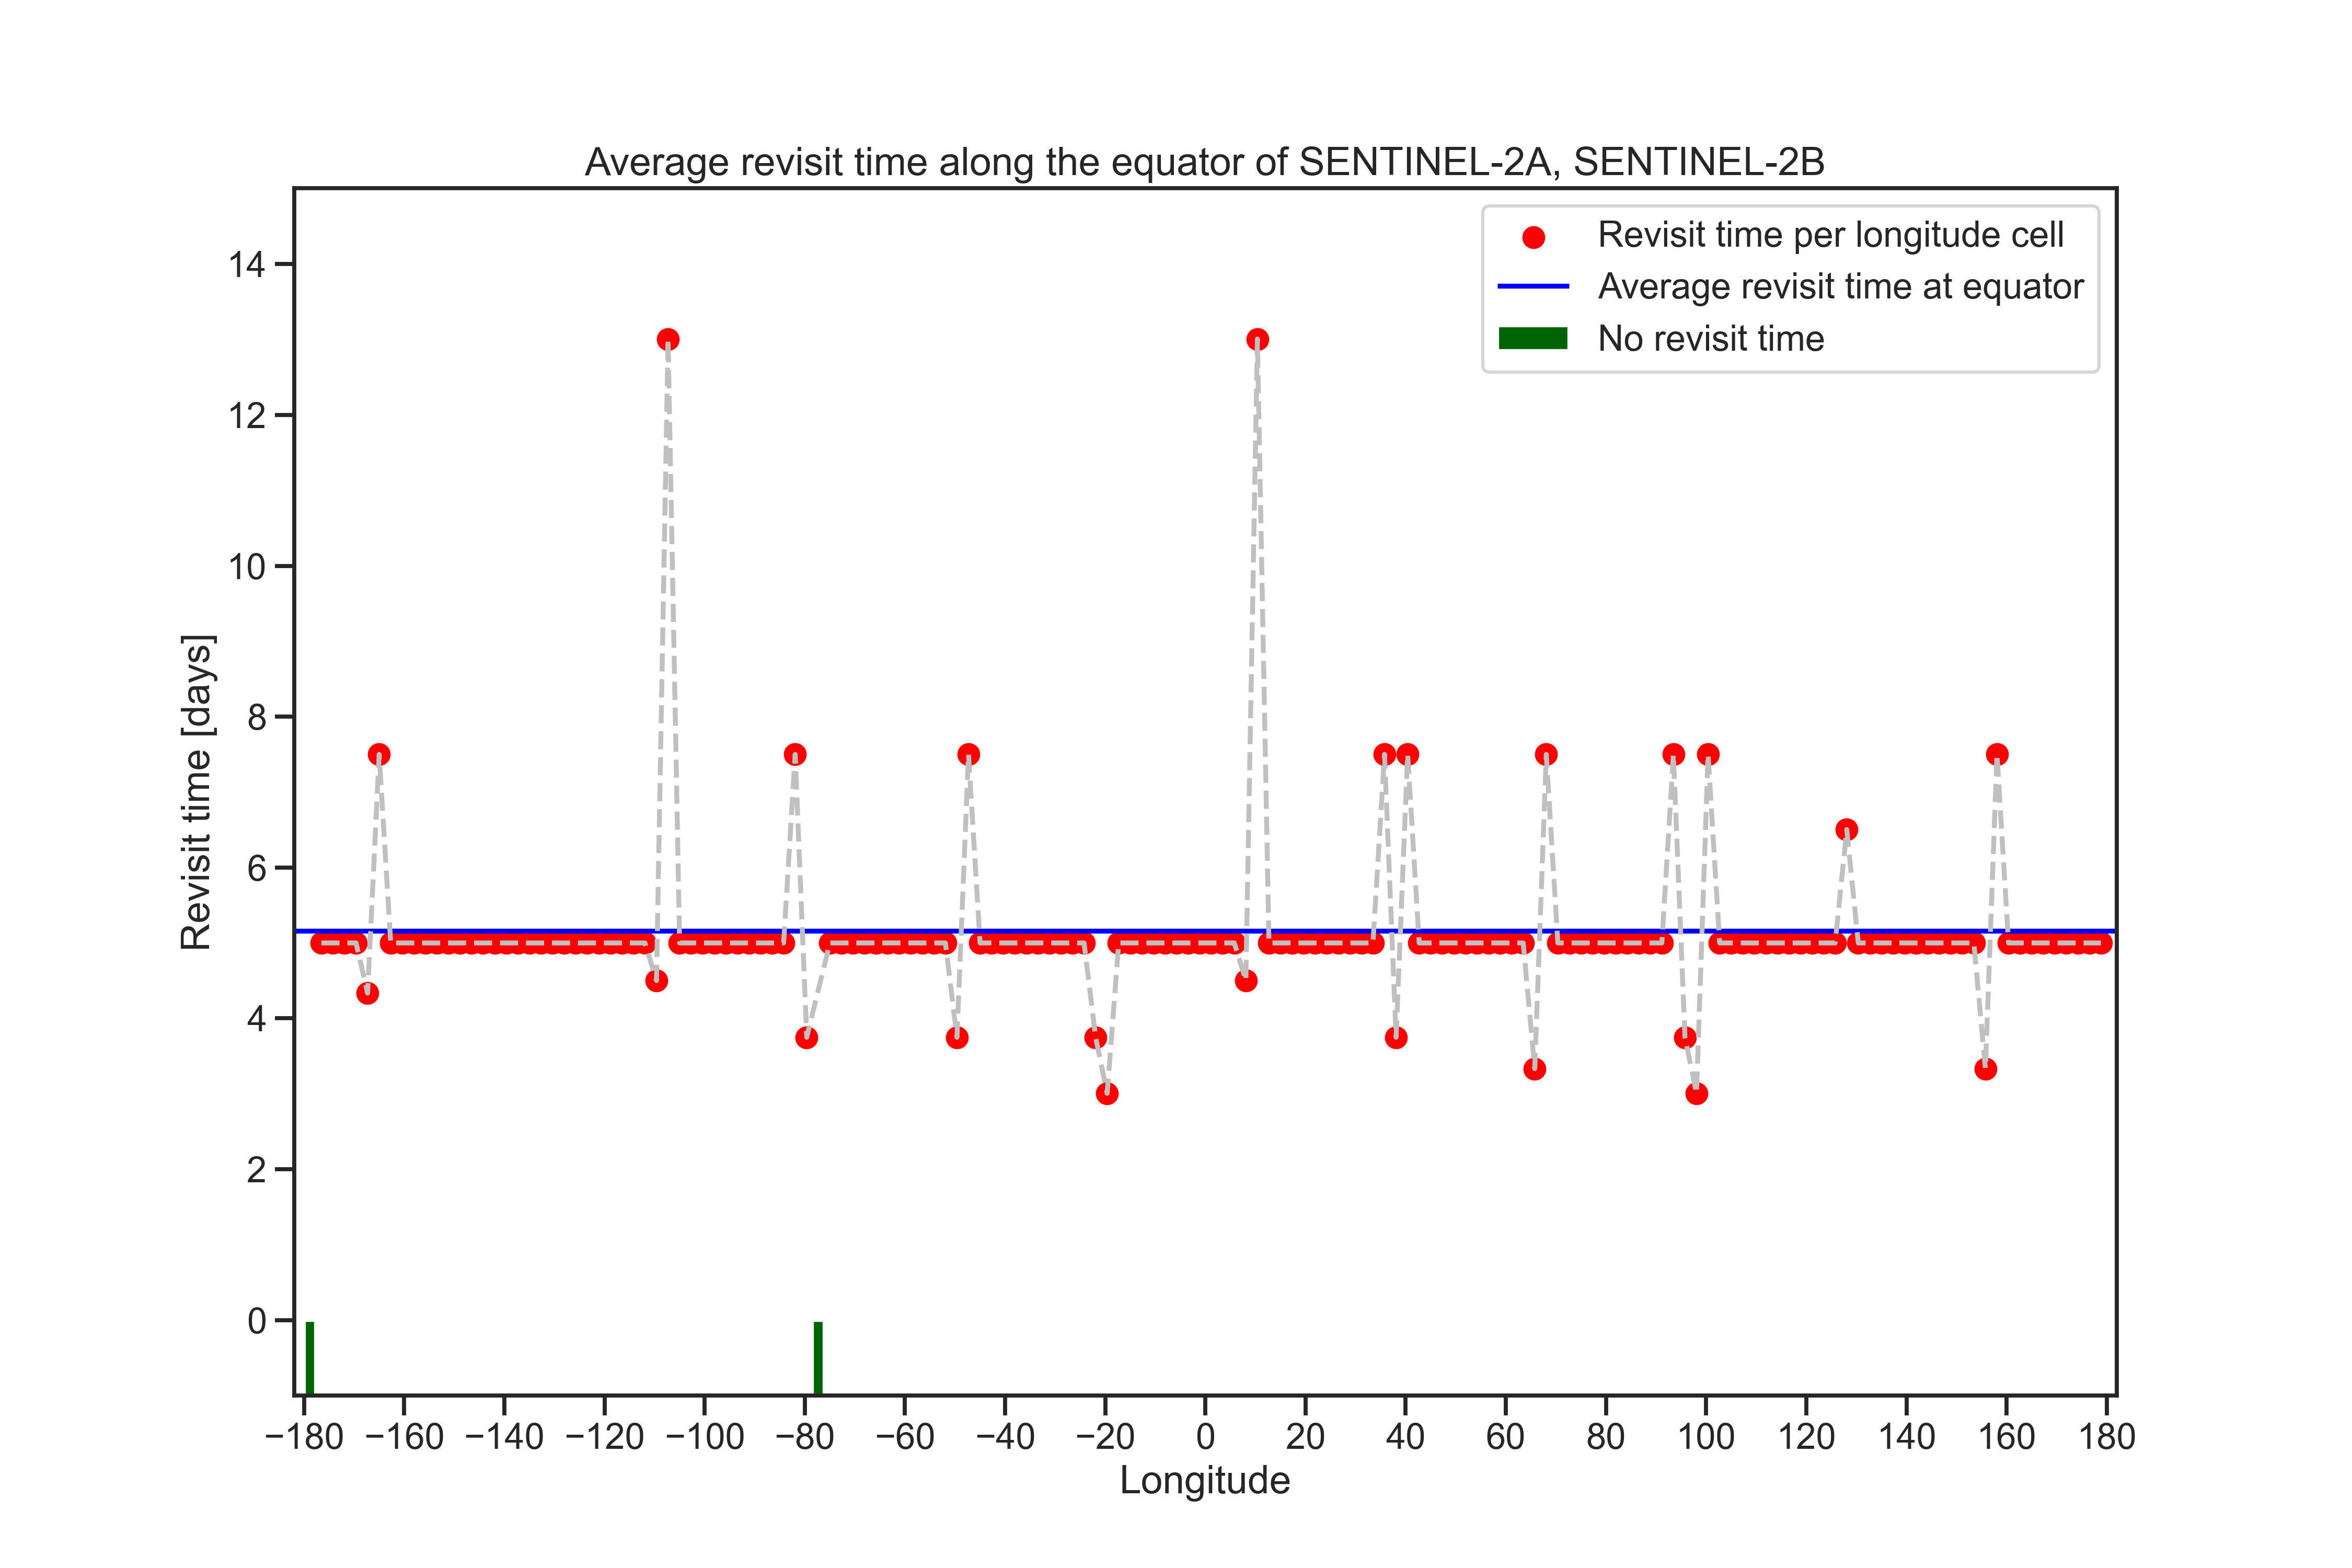
\includegraphics[width=0.9\textwidth]{Images/revisit_time_of_SENTINEL-2A_SENTINEL-2B.png}
\caption{Average revisit time per longitude cell along the equator of the Sentinel-2 constellation. The length of the longitude cell was determined based on the swath width of the satellite's sensor, which in this case is 290 km. The average revisit time at the equator of Sentinel-2A and Sentinel-2B is 5.16 days.}
\label{revisit_time_of_SENTINEL-2A_SENTINEL-2B}
\end{figure}

\begin{figure}
\centering
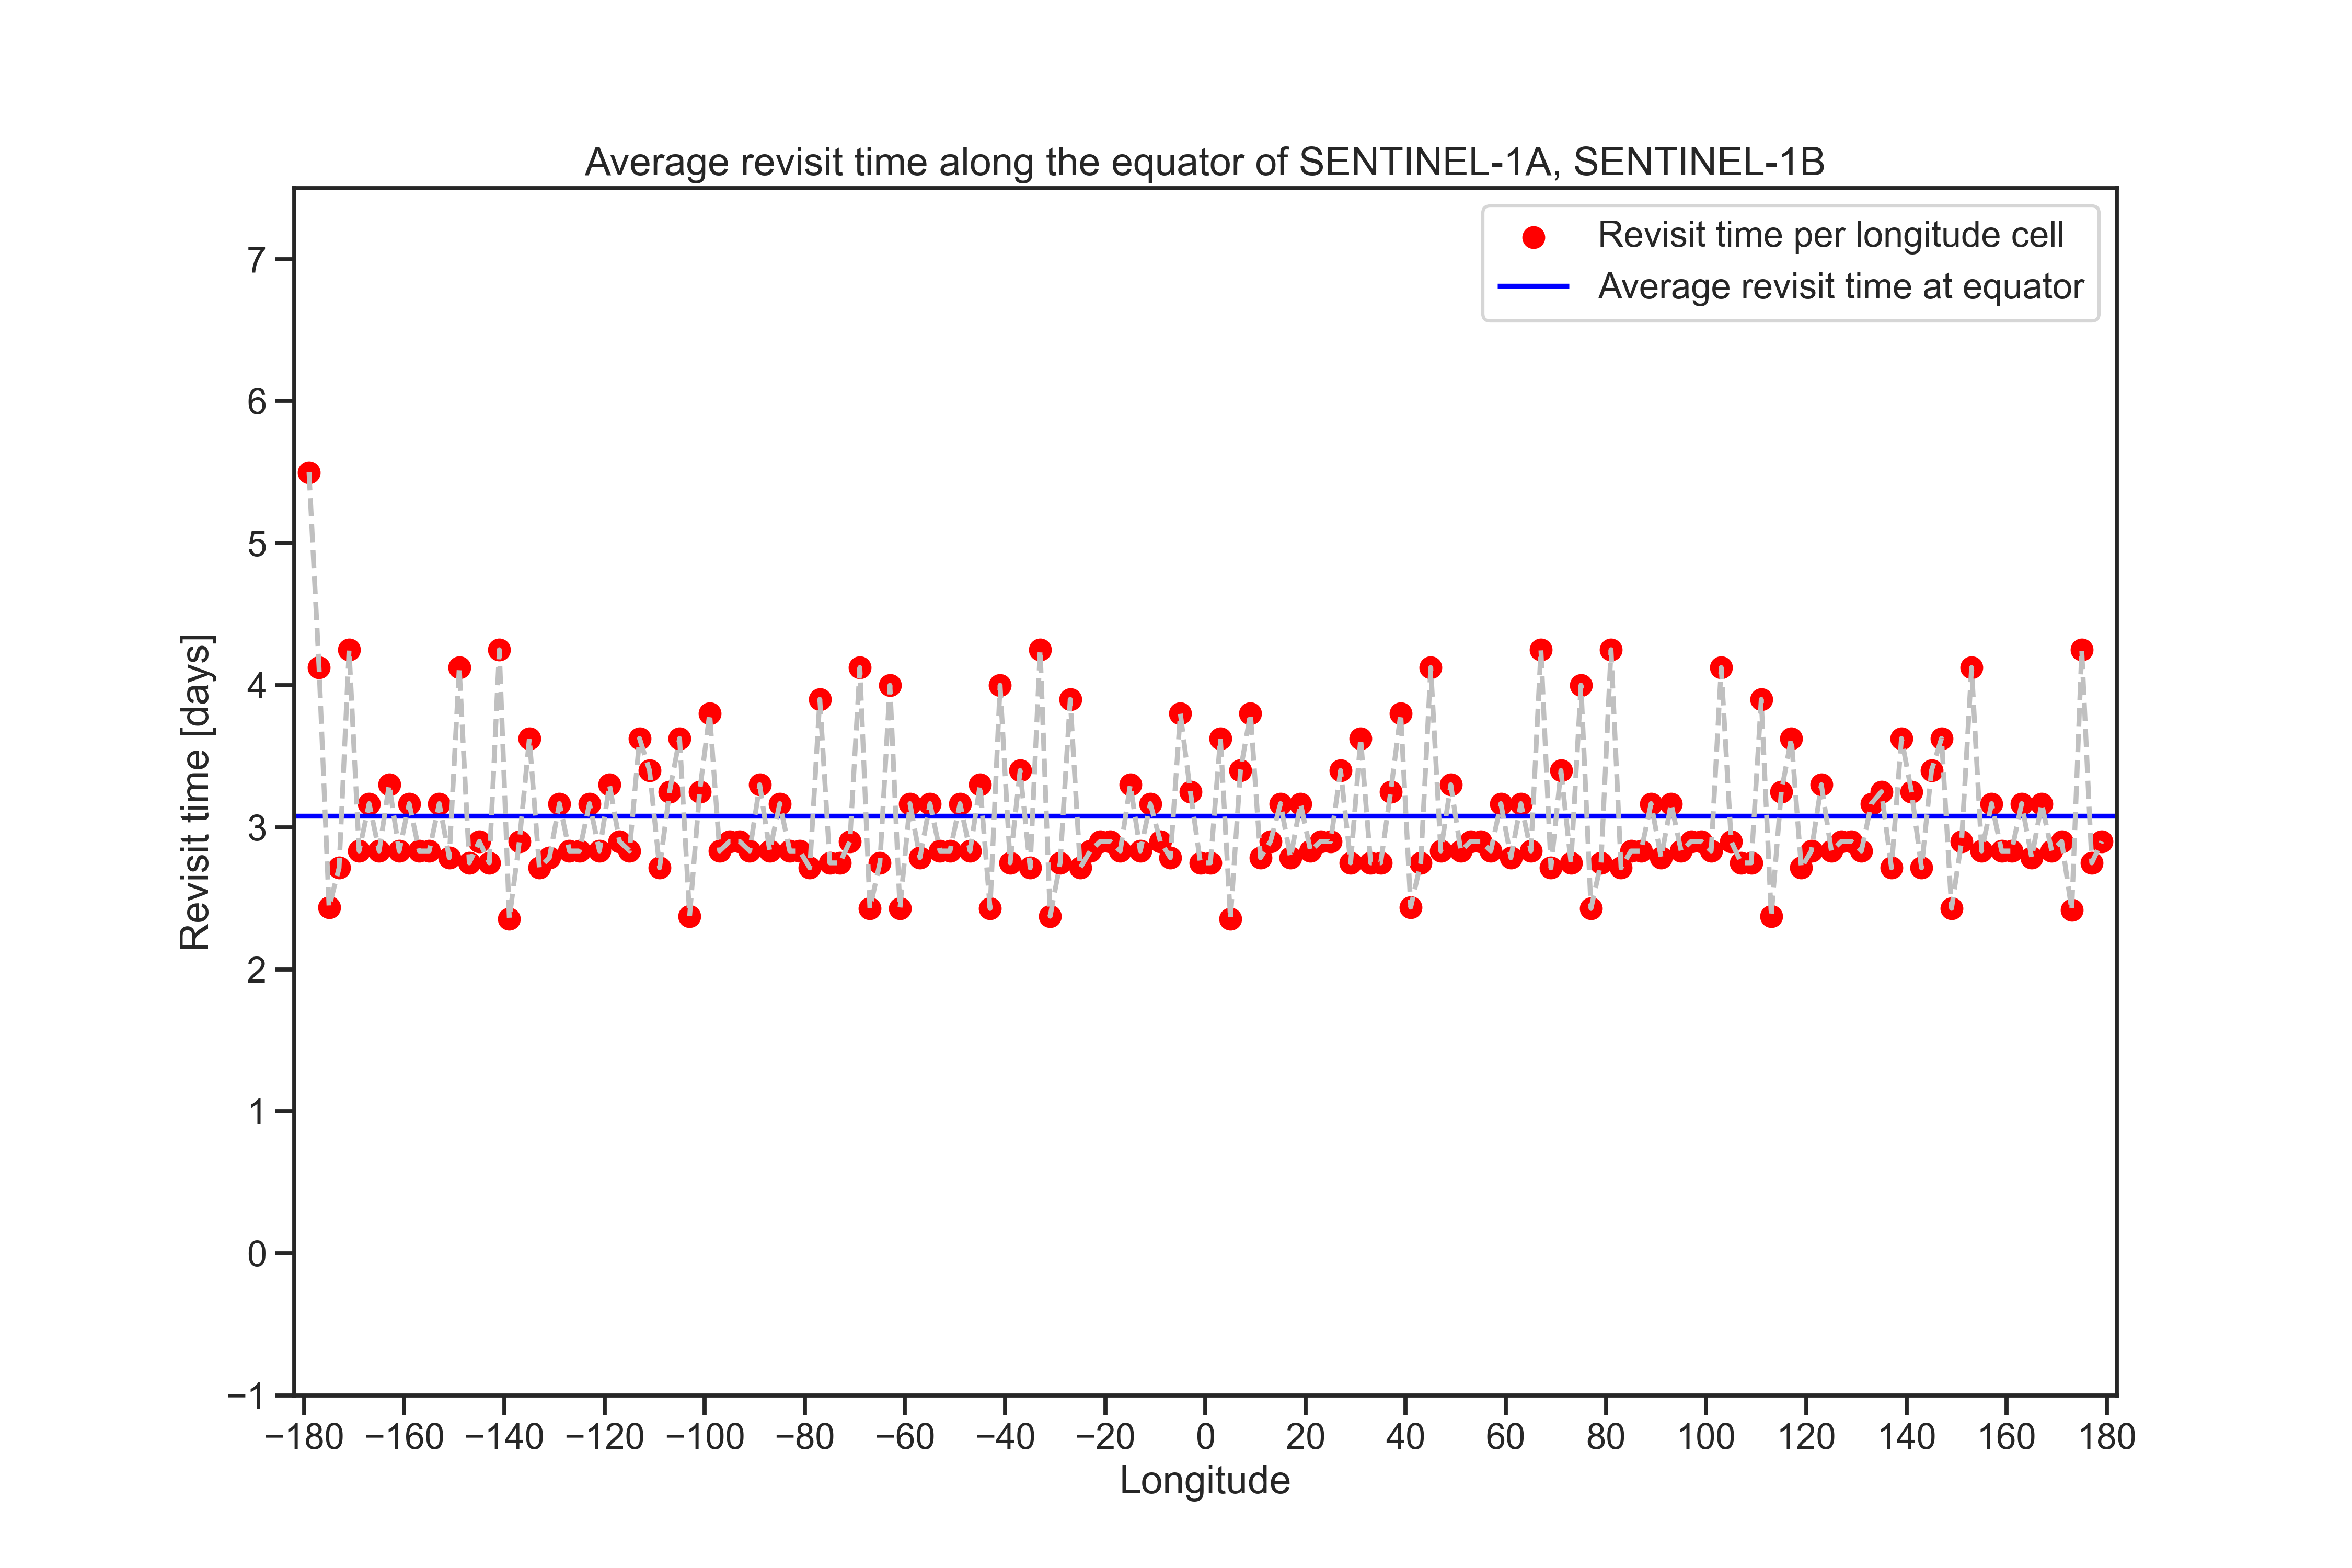
\includegraphics[width=0.9\textwidth]{Images/revisit_time_of_SENTINEL-1A_SENTINEL-1B.png}
\caption{Average revisit time per longitude cell along the equator of the Sentinel-1 constellation. The length of the longitude cell was determined based on the swath width of the Interferometric Wide Swath Mode, which is 250 km. The average revisit time at the equator of Sentinel-1A and Sentinel-1B is 3.08 days.}
\label{revisit_time_of_SENTINEL-1A_SENTINEL-1B}
\end{figure}

Furthermore, the user can also find out what is the number of the crossing times of the satellite above the Earth's cells. As an example, the Sentinel-1 constellation for a simulation of 20 orbits is presented in Figure \ref{SENTINEL-1A_SENTINEL-1B_crossing_times.png} for showing this application's feature.

\begin{figure}
\centering
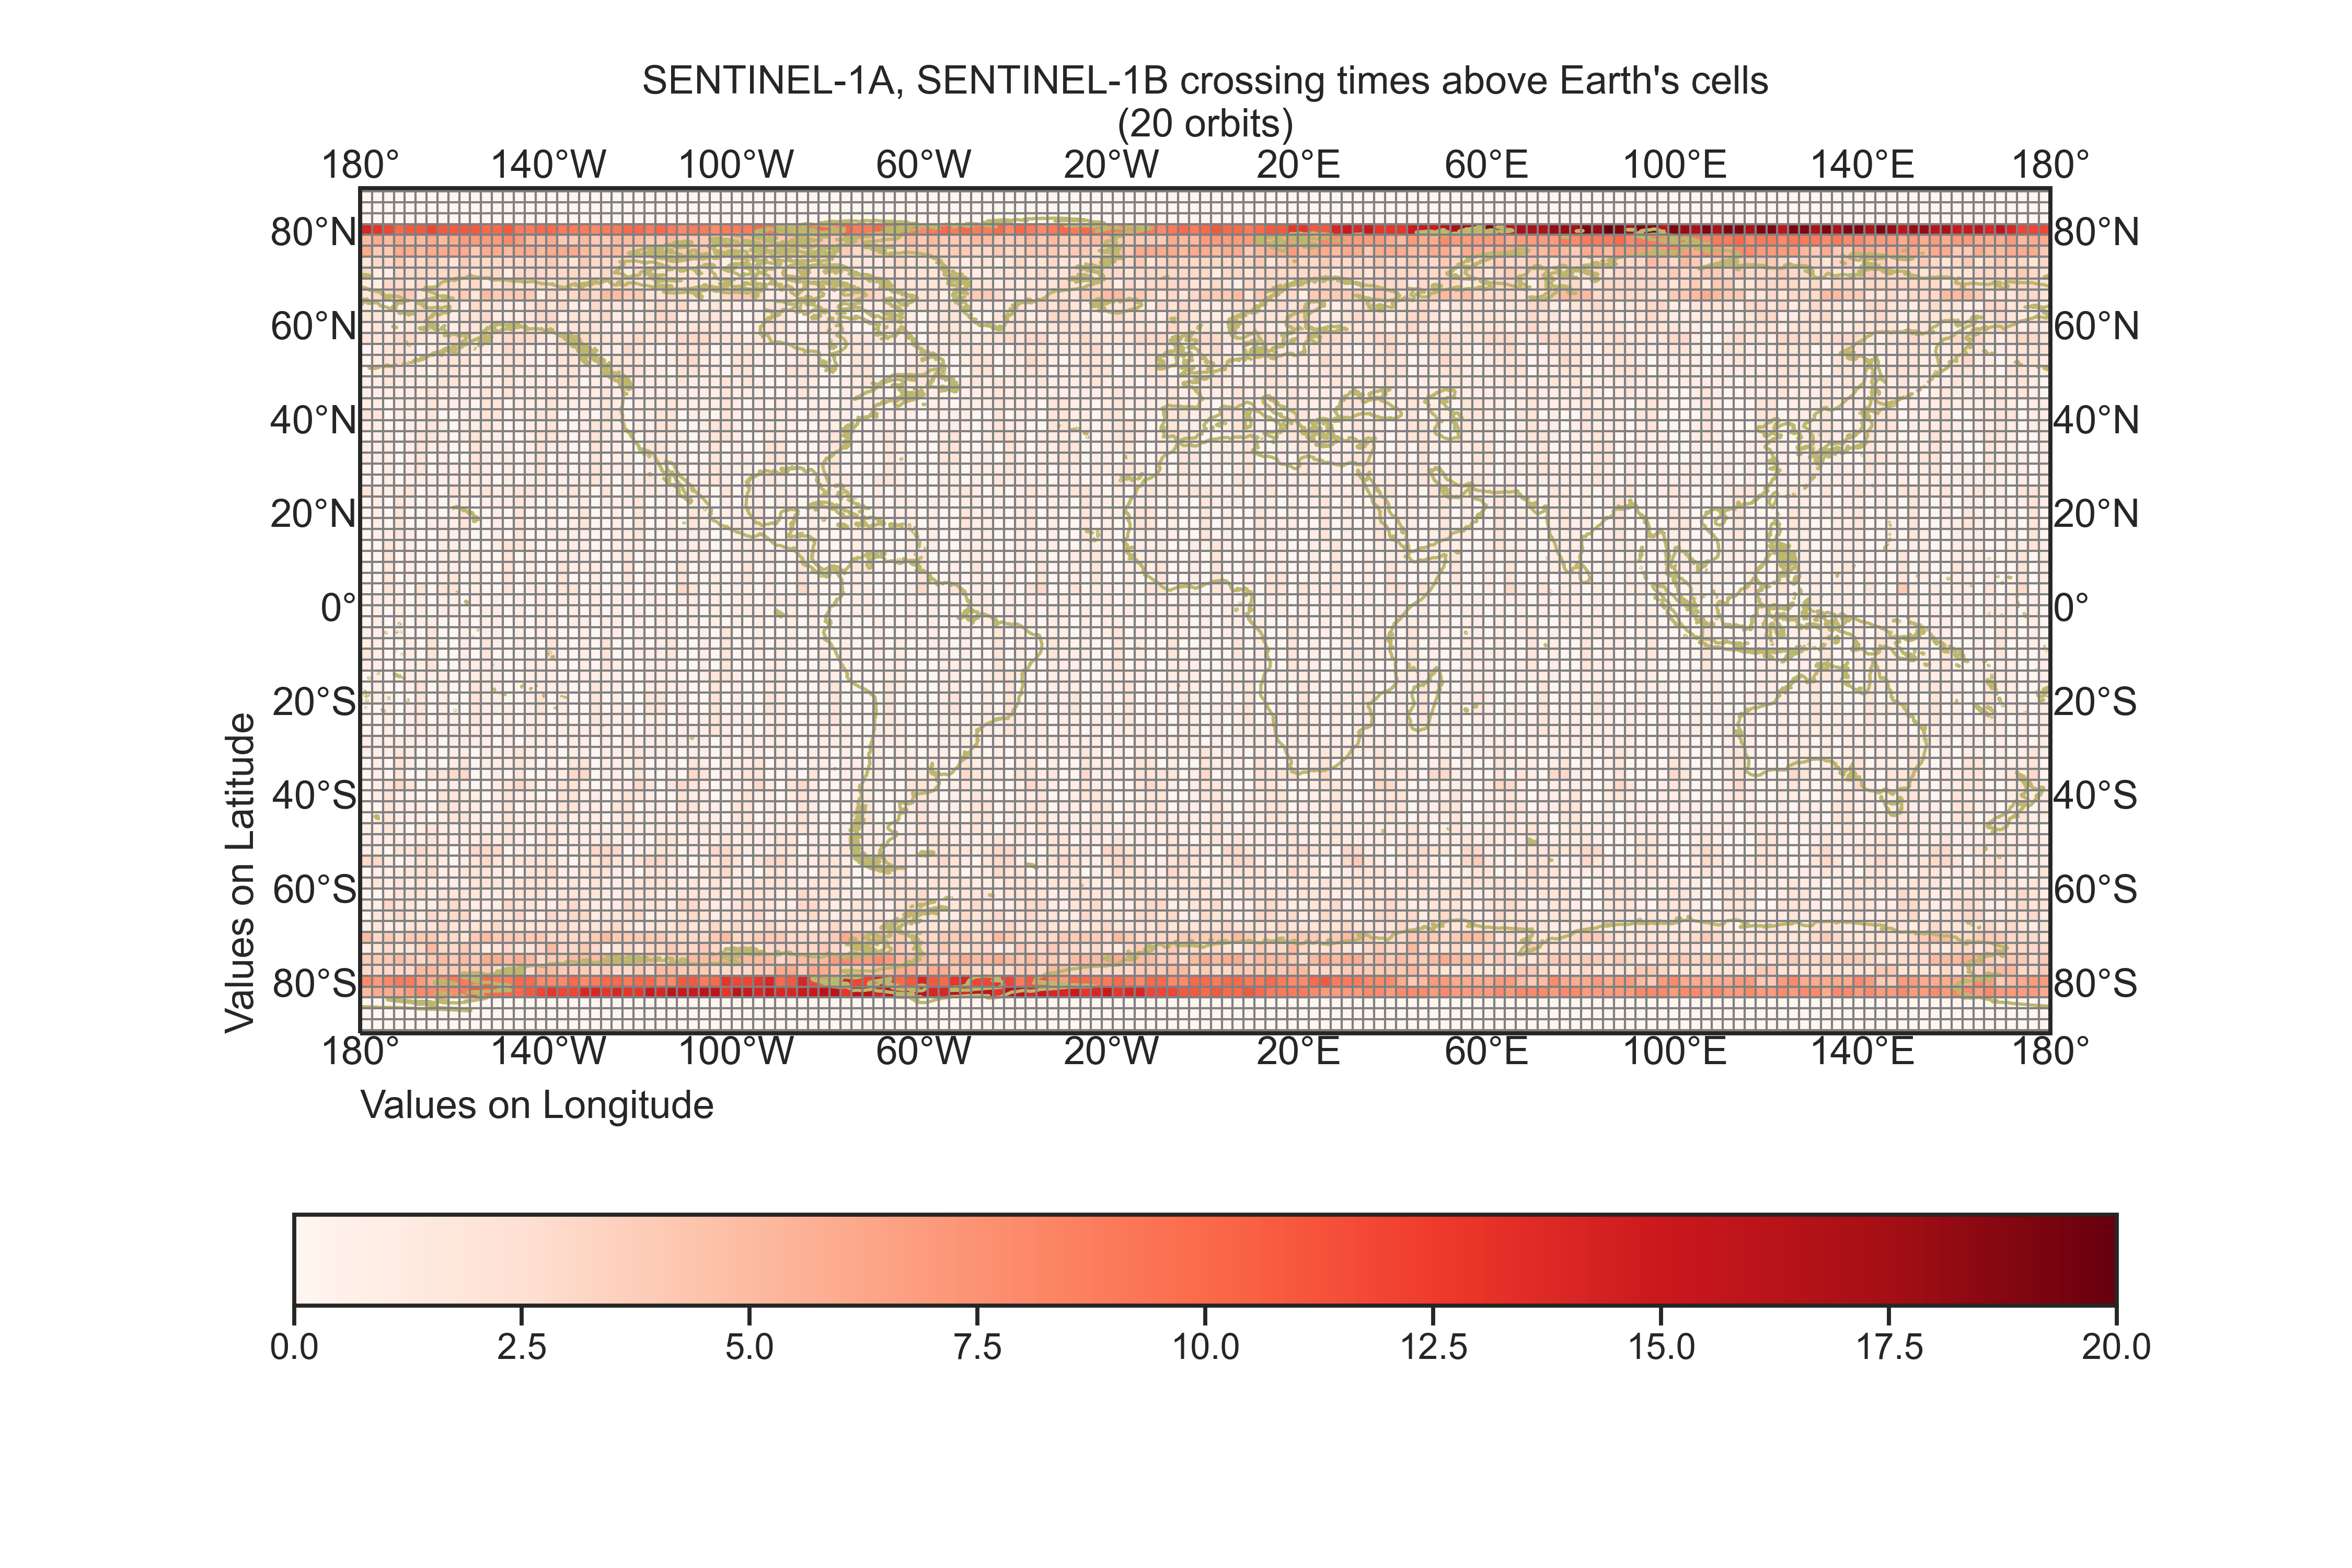
\includegraphics[width=0.9\textwidth]{Images/SENTINEL-1A_SENTINEL-1B_crossing_times.png}
\caption{The number of crossing times of the Sentinel-1 constellation above the Earth's cells. The creation of the cells was determined based on the swath width of the satellite's sensor.}
\label{SENTINEL-1A_SENTINEL-1B_crossing_times.png}
\end{figure}
% Run main_code_db_aggregated.py for Sentinel2A,B. BE CAREFUL in code you should have: type_of_sensor = 'active' !! This is because if the satellite is passive then, the groundtrack will be depicted only in the descending passes and it will be half!

% (If I want to create an aggregated revisit time of satellites, which have different swath widths, then a safe solution would be to use the maximum swath width of all of them and use it globally - since we need to have the same - there is one table with specific dimensions calculating the revisit time- and thus cells with certain grid interval. If I use the minimum swath width of the swath widths that the group of satellites have, then it might happen that some of the satellites do not produce an outcome of revisit time in this specific -and smaller than theirs- swath width. So, to be on the safe side - use the max swath width among all).

\bigskip
\section{Investigation of orbital characteristics of new satellite for a more frequent revisit time}
\bigskip

A user has also the possibility to find the position of a new satellite, which can achieve together with a group of other satellites a more frequent revisit time. As a first experiment, the Sentinel-2 constellation was used. Then, a prospective new satellite with similar orbital characteristics to the Sentinel-2 satellites was used to calculate the overall revisit time. The parameter that is varying is the mean anomaly ($M$), which means that the position of the prospective satellite in the orbital plane is changing throughout the different cases. The revisit time at the equator was then found for every case as it can be seen in Figure \ref{revisit_time_ofdoubleaxis_SENTINEL-2A_SENTINEL-2B_Example-satellite}. The two vertical green lines indicate the position of the Sentinel-2A and Sentinel-2B  in the orbital plane. Additionally, the reduction of the revisit time that the addition of the Example-satellite has brought is shown in the right side y-axis.

% Take Sentinel-2A and 2B. Think of a similar satellite with similar altitude, that its position varies (true anomaly varies - at the beginning ..? probably...) --> the position along the orbit. What is the position of the new satellite that has the maximum (the most often) revisit time?

\begin{figure}
\centering
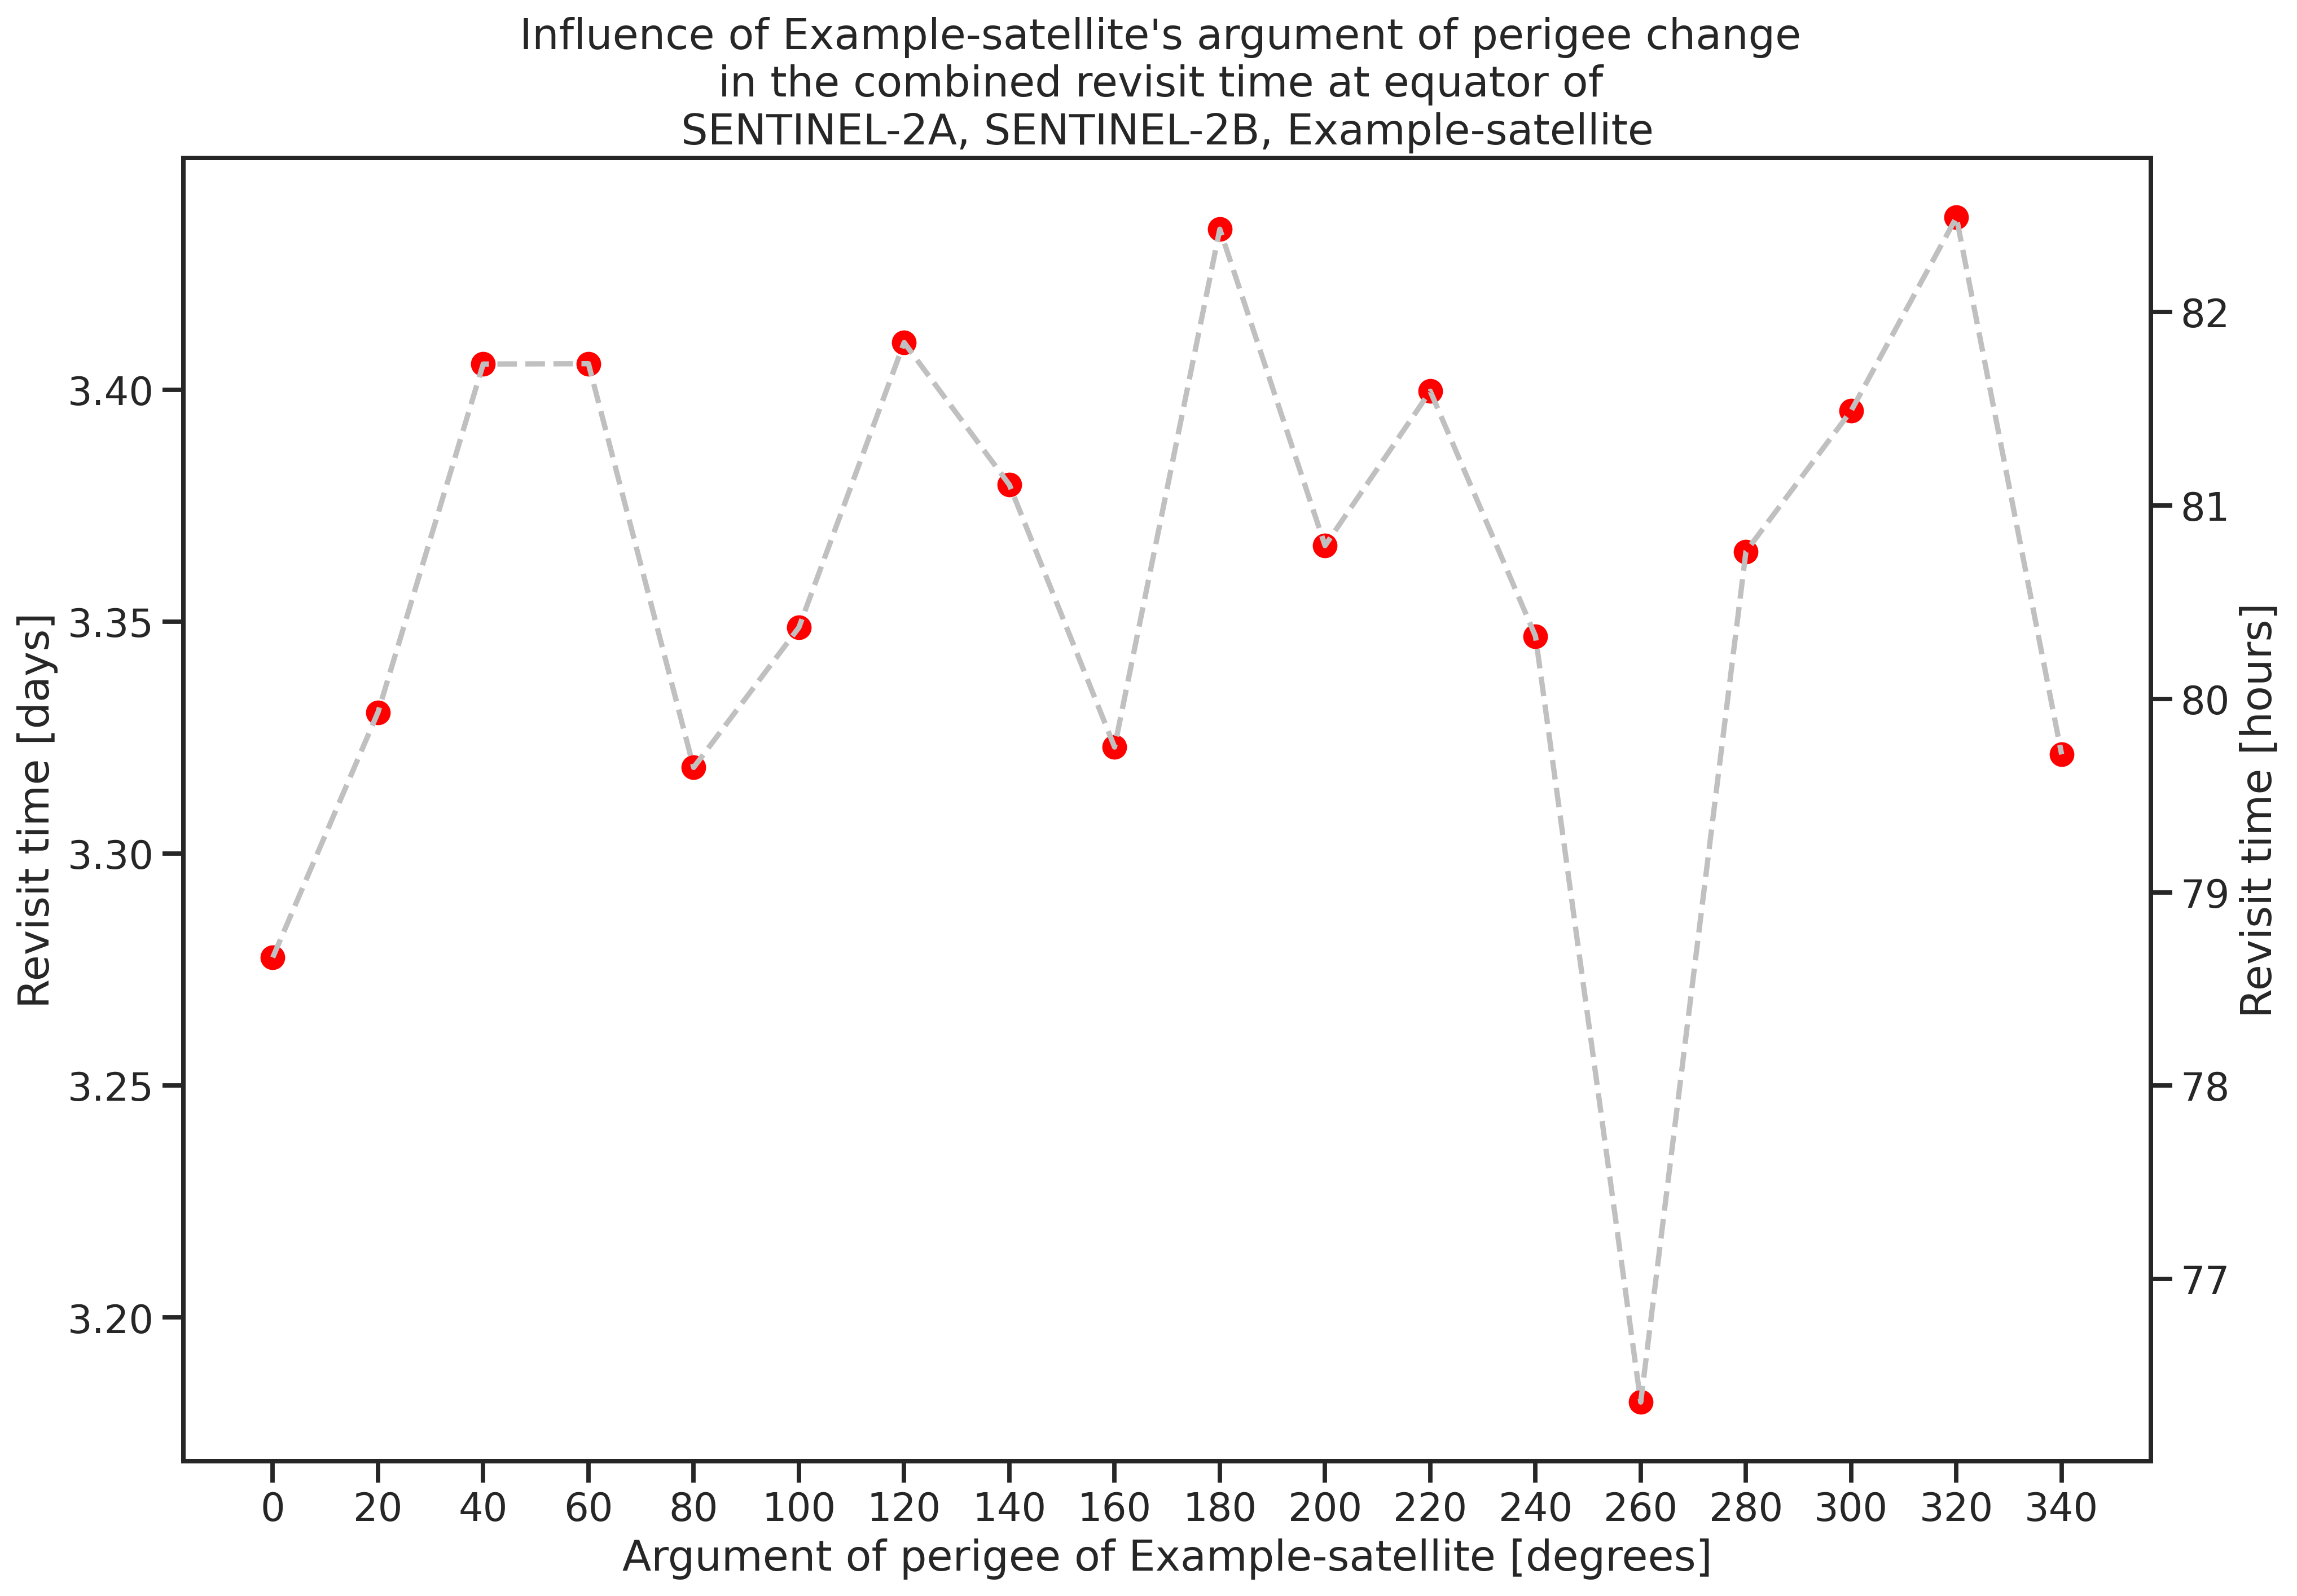
\includegraphics[width=0.9\textwidth]{Images/revisit_time_ofdoubleaxis_SENTINEL-2A_SENTINEL-2B_Example-satellite.png}
\caption{Influence of the new satellite's mean anomaly change in the combined revisit time at equator of the Sentinel-2 constellation and this new Example-satellite. The green lines indicate the position of the Sentinel-2A and 2B satellites in the orbital plane.}
\label{revisit_time_ofdoubleaxis_SENTINEL-2A_SENTINEL-2B_Example-satellite}
\end{figure}

% The Sentinel-2A has mean anomaly: 93.2879064 degrees
% The Sentinel-2B has actually: 281.5507975, but in the figure we show mean anomaly: 275.5507975
% The Example-satellite's mean anomaly is varying. However when we plug in the database 0degrees, this is translated as 180.786359degrees, which we plot in this figure as 180degrees.

% Code: main_code_db_aggregated_experiment_Sent2.py
% The differences of this code with "code_db_aggregated.py" are: 1. Big "for loop" at the beginning with change_omega (BE CAREFUL TO BE CORRECT)., 2. In the determination of omega (line 204 or line 207) change it! If id == 249: (Here is the id of the Example_satellite), 3. I have set the list "multiple_average_aggregated_zerolat_without0", 4. I append the revisit time there (line 1072), 5. Change the "argument_of_perigee" parameter to have the correct amount of numbers + Make sure that all the id (satellites) that I use in the code are inside the database in the VE!!! If not update the database in VE.

A similar procedure of finding the optimal altitude of a new satellite was also implemented. The Sentinel-2 constellation was also part of this experiment and as it was calculated, its average altitude is around 790 km. Then, the prospective satellite with similar orbital characteristics was created in order to calculate the overall revisit time when its altitude is varying. This new satellite was also assumed to be in a Sun-synchronous orbit as the Sentinel-2 constellation. The range of the different altitudes that were tested were 20 km below and above the average altitude. This range was found based on the fact that the period of the satellite is not changed substantially and thus in accordance with the inclination, the orbit is maintained a Sun-synchronous one.

The experiments of finding the overall revisit time with the altitude change of this Example's satellite were performed for three different positions of the Example satellite in the orbital plane. Those positions, or else the values of the mean anomaly of the Example satellite for every case, were selected from the previous Figure in order to be ensured that the position of the third satellite will not be co-located with one of the two existing ones. For this reason, as can be seen in Figure \ref{revisit_time_ofdoubleaxis_SENTINEL-2A_SENTINEL-2B_Example-satellite}, the mean anomaly of the Sentinel-2A and 2B for the starting epoch of the simulation is approximately 93 and 273 degrees respectively. As a result, the three example cases that are presented, show the overall revisit time with the altitude change of the Example satellite when its mean anomaly is 50, 180 and 330 degrees (Figures \ref{revisit_time_ofdoubleaxisaltitude_SENTINEL-2A_SENTINEL-2B_Example-satellite_50deg}, \ref{revisit_time_ofdoubleaxisaltitude_SENTINEL-2A_SENTINEL-2B_Example-satellite_180deg}, \ref{revisit_time_ofdoubleaxisaltitude_SENTINEL-2A_SENTINEL-2B_Example-satellite_330deg}).

% I assume that the orbit is maintained as SSO (as I said).
% Source no1: wikipedia page of SSO. I used the equation of cos(i)=... by changing the semimajor axis according to the change of altitude. However, an "acceptable/ official" source to mention is Vallado4thedit p.890, Equation: 11-14
% Then, based on the graph that is in the pdf "2019_Joint_Agency_Commercial_Imagery_Evaluation" in p.15, I checked whether the value of the inclination is not on the line. This graph shows the relationship between inclination and time period in order the orbit to be maintained SSO.

\begin{figure}
\centering
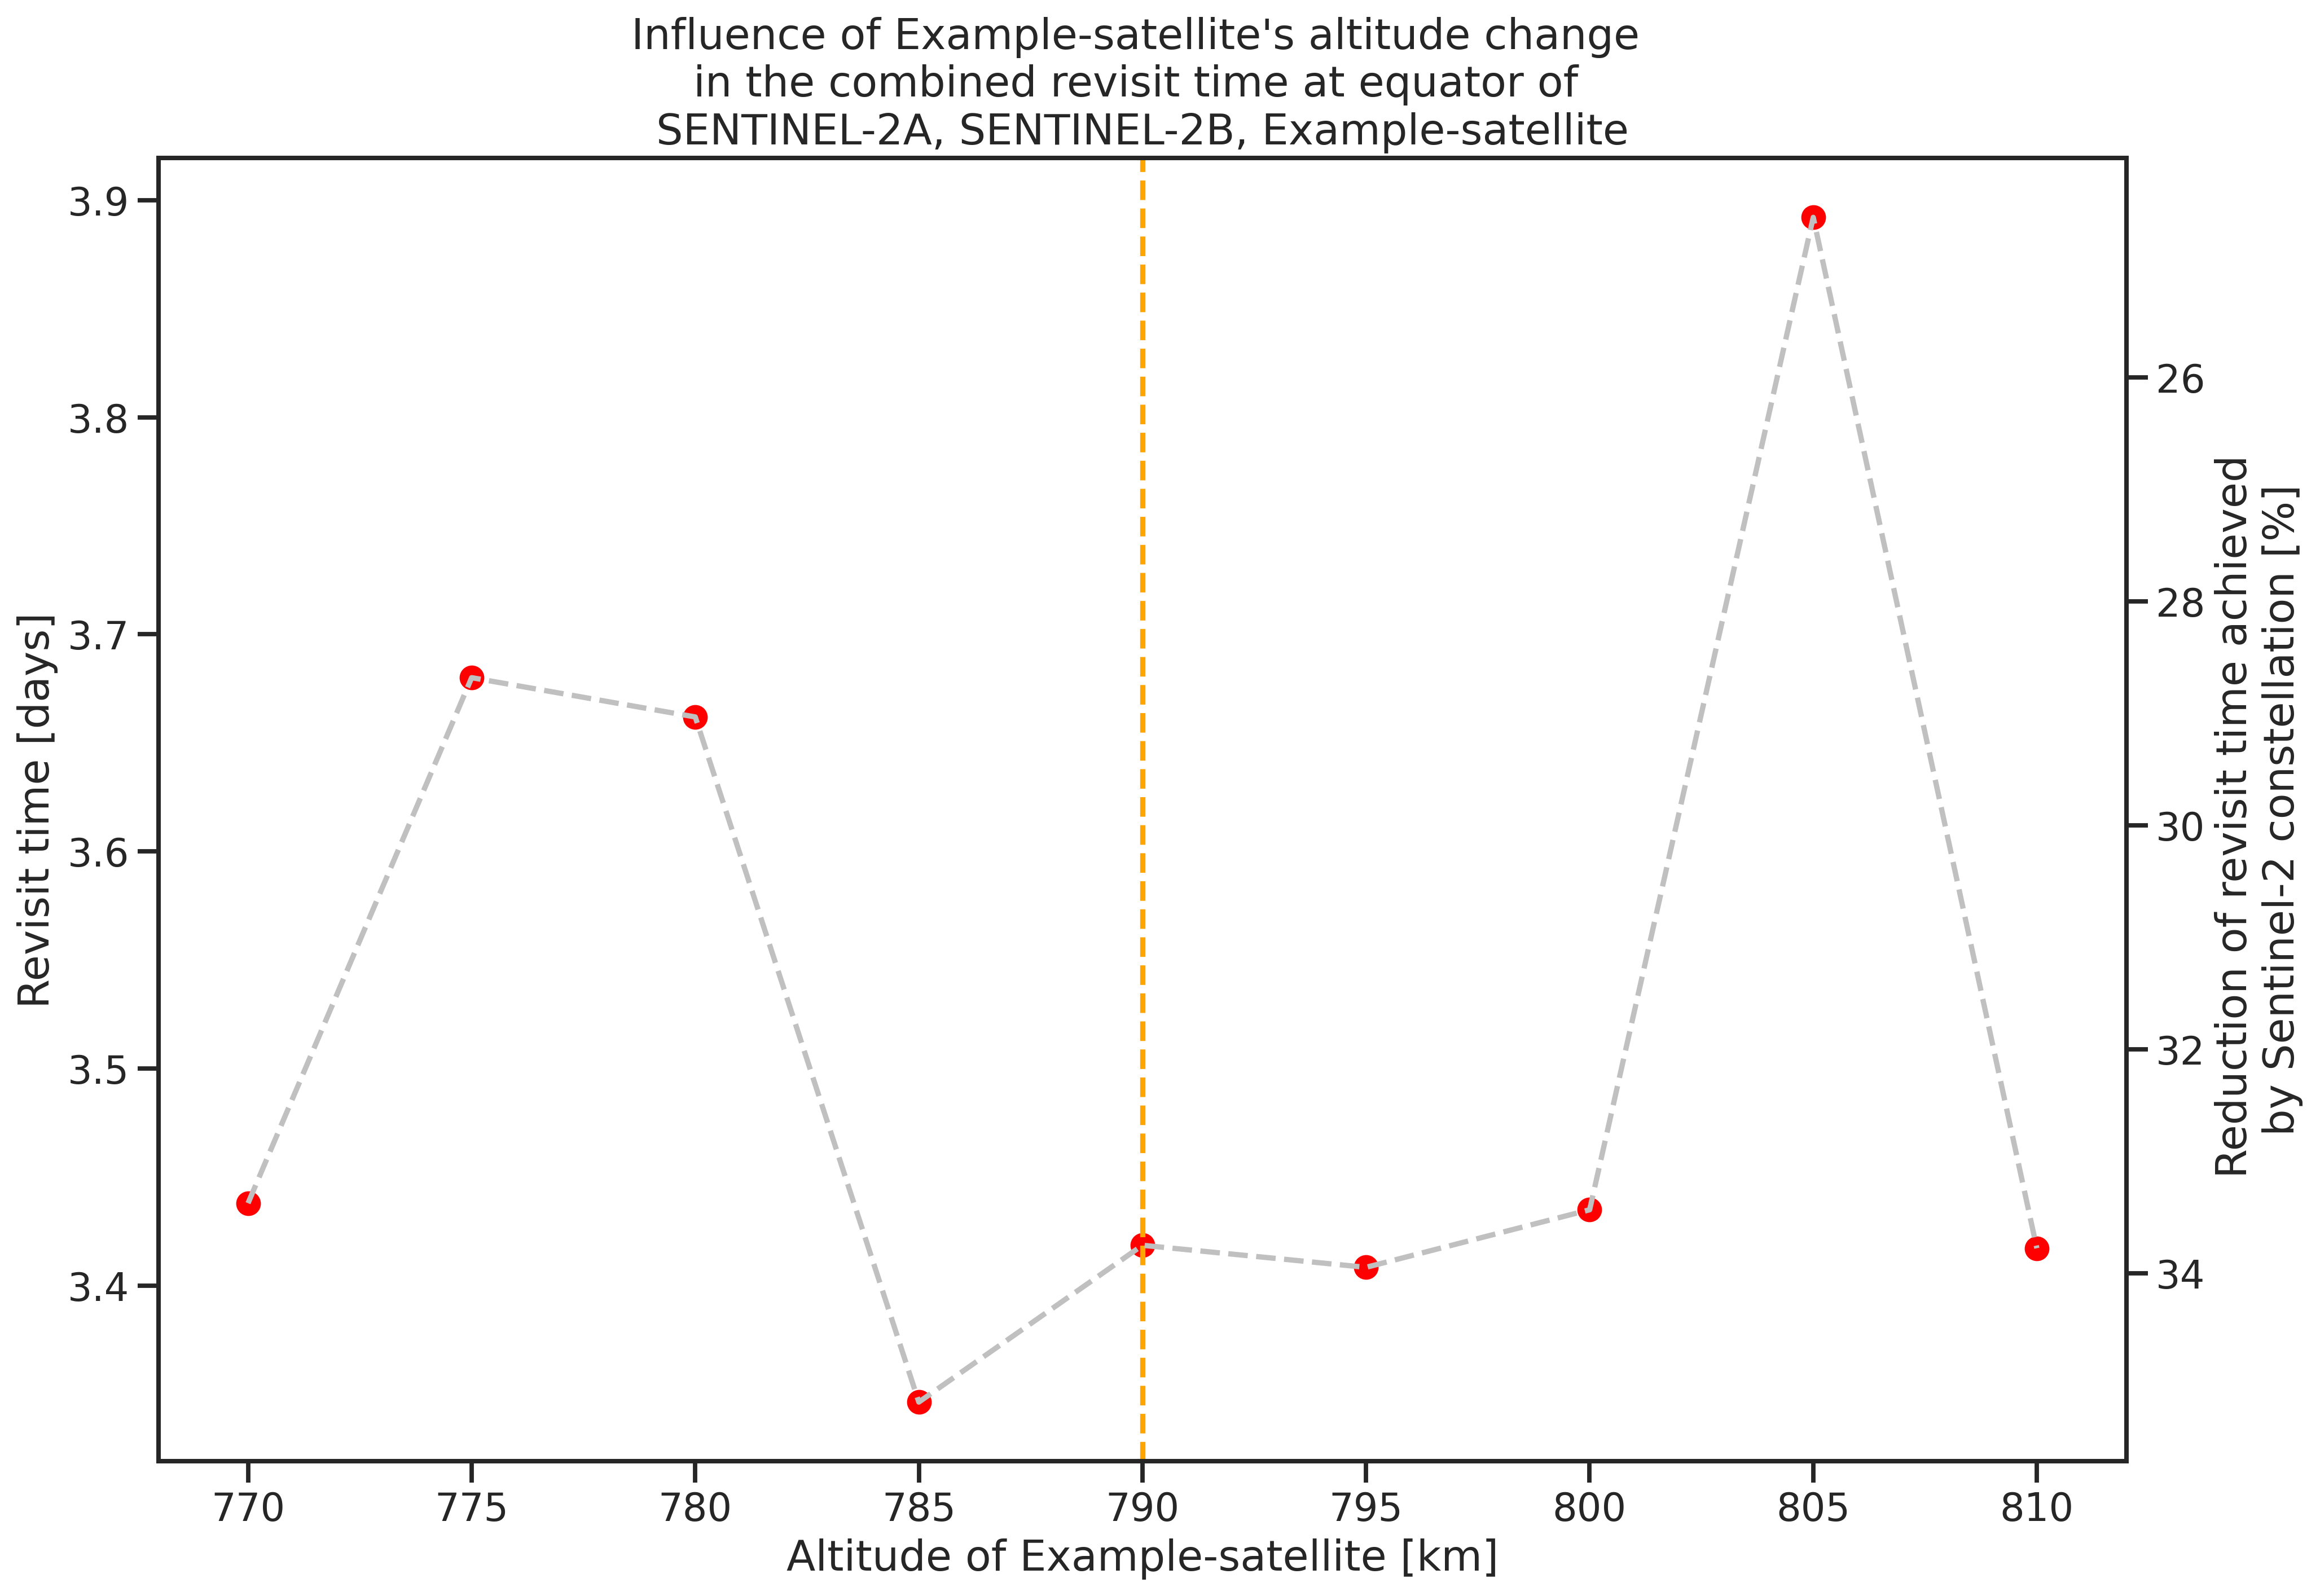
\includegraphics[width=0.9\textwidth]{Images/revisit_time_ofdoubleaxisaltitude_SENTINEL-2A_SENTINEL-2B_Example-satellite_50deg.png}
\caption{Influence of the new satellite's altitude change in the combined revisit time at equator of the Sentinel-2 constellation and the Example-satellite. The yellow line indicates the altitude of the satellites of the Sentinel-2 constellation. \underline{The mean anomaly of the Example satellite is 50 degrees.}}
\label{revisit_time_ofdoubleaxisaltitude_SENTINEL-2A_SENTINEL-2B_Example-satellite_50deg}
\end{figure}

\begin{figure}
\centering
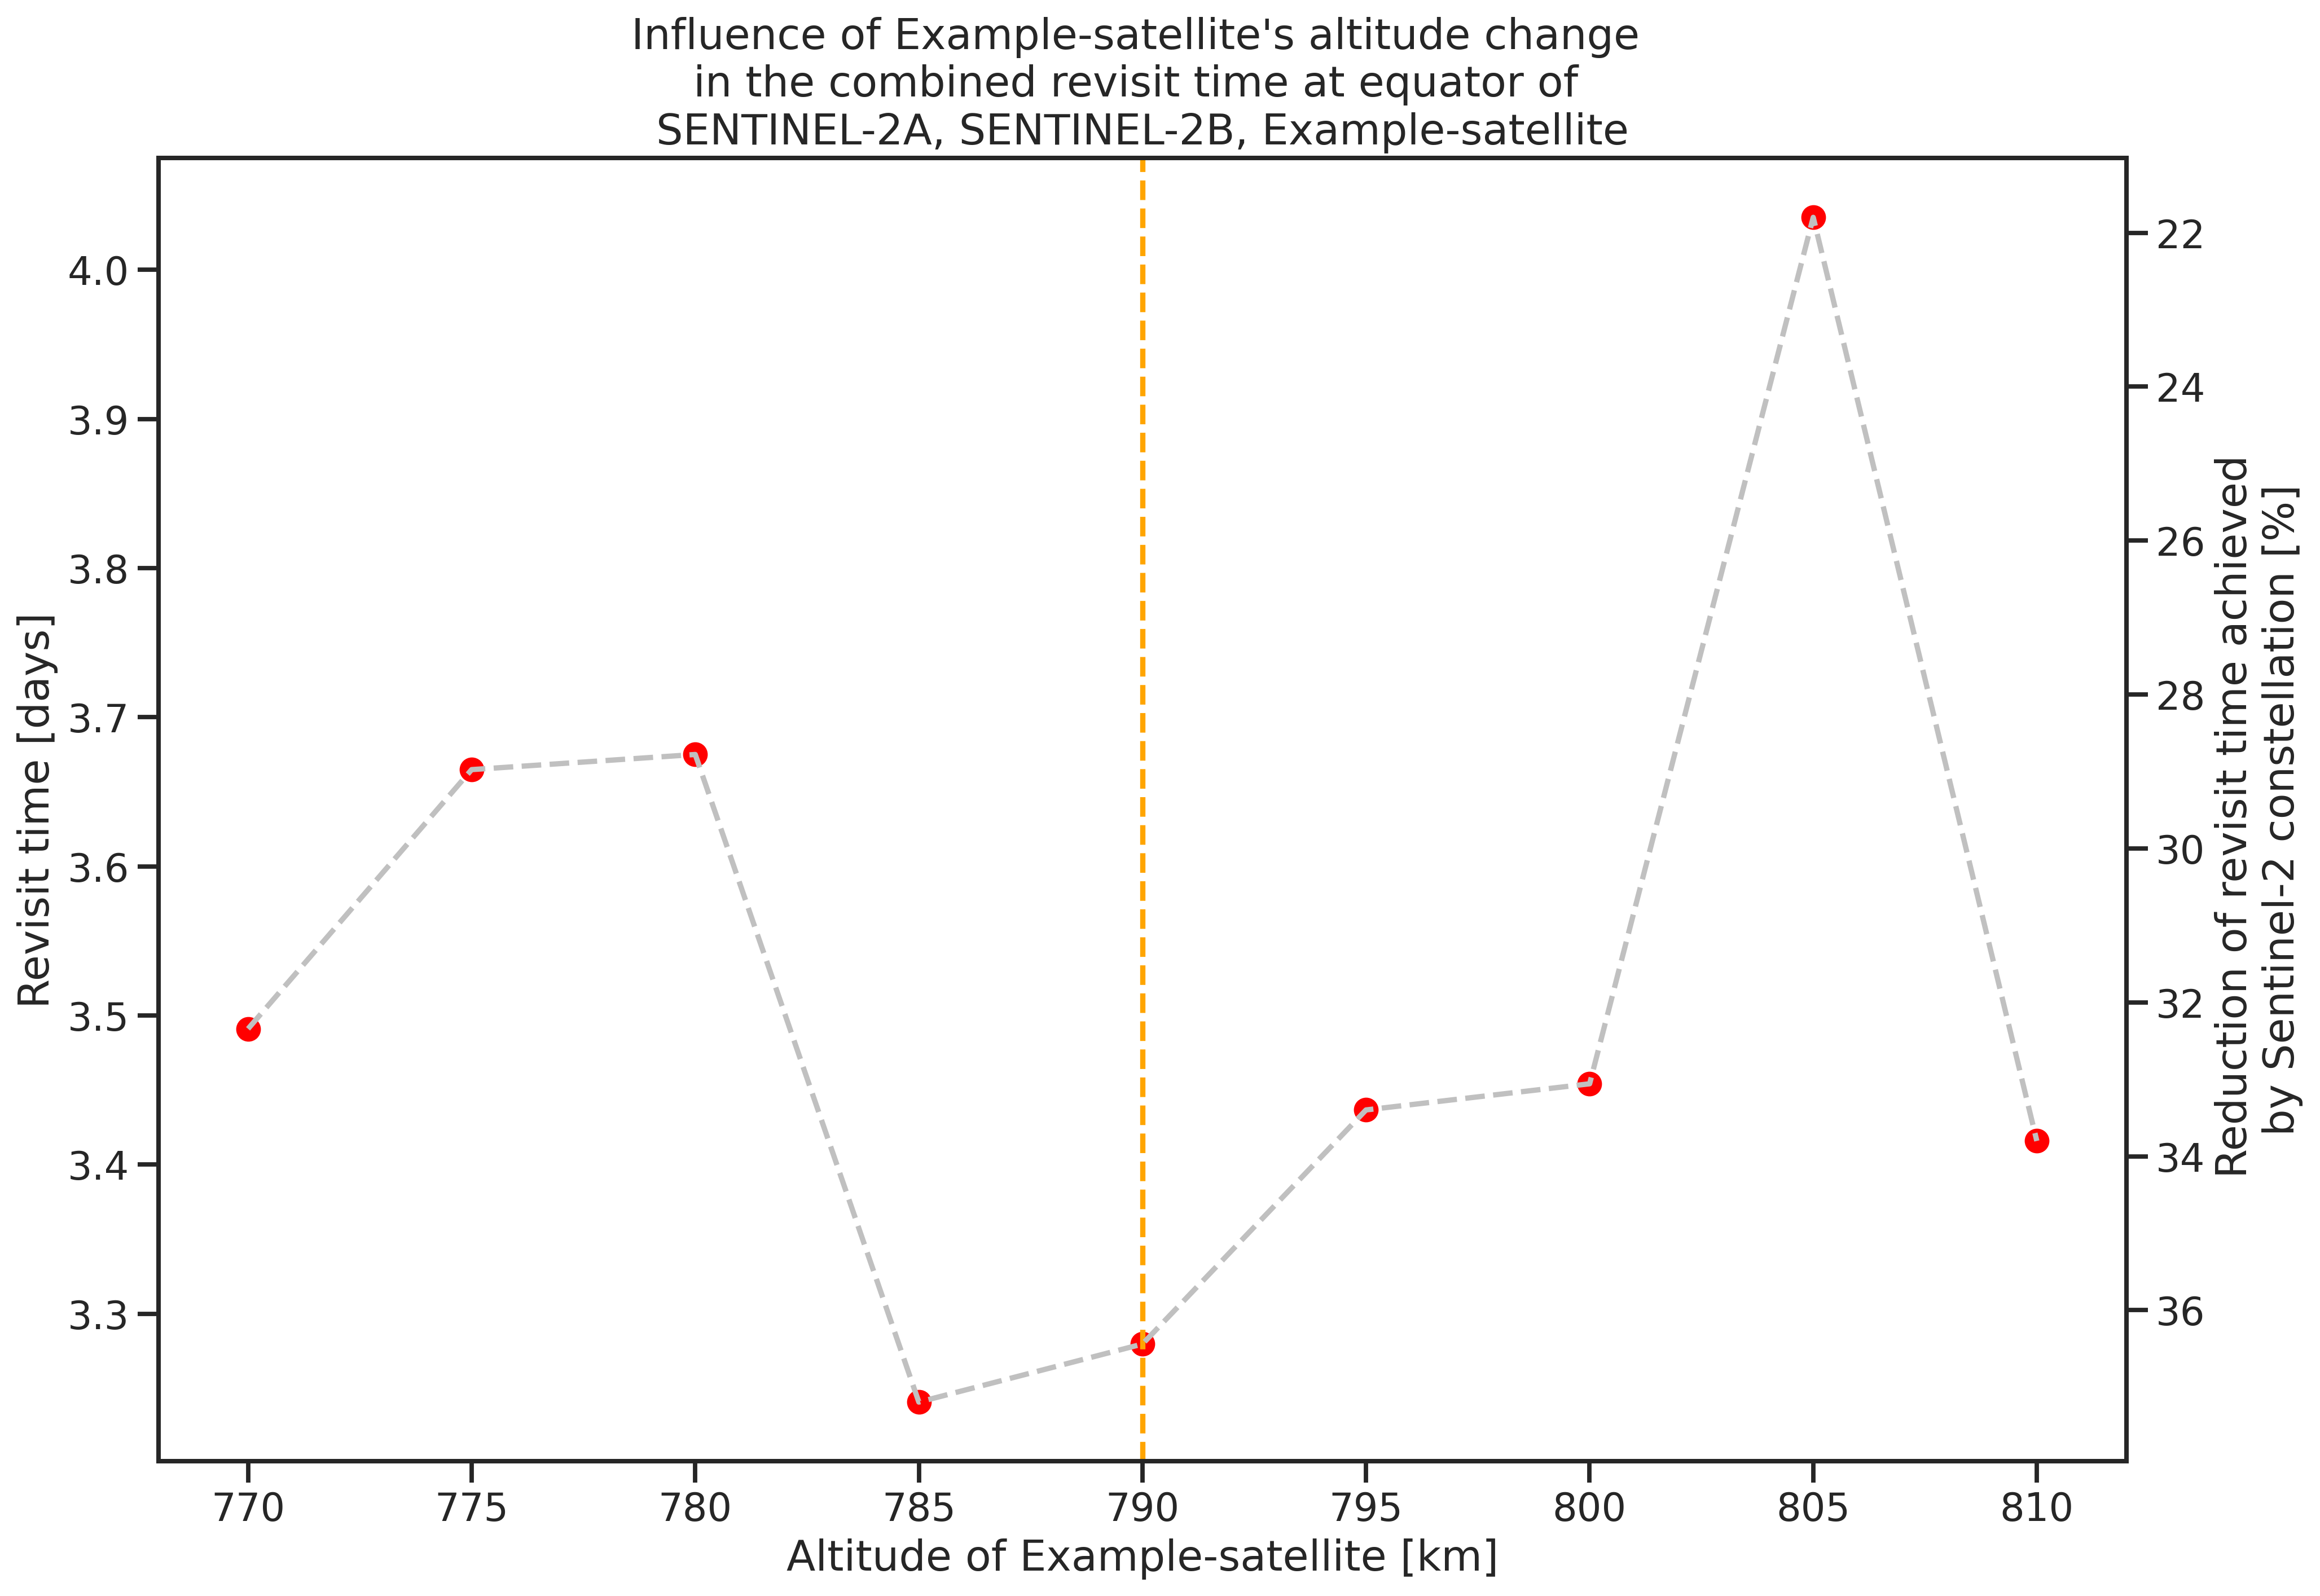
\includegraphics[width=0.9\textwidth]{Images/revisit_time_ofdoubleaxisaltitude_SENTINEL-2A_SENTINEL-2B_Example-satellite_180deg.png}
\caption{Influence of the new satellite's altitude change in the combined revisit time at equator of the Sentinel-2 constellation and the Example-satellite. The yellow line indicates the altitude of the satellites of the Sentinel-2 constellation. \underline{The mean anomaly of the Example satellite is 180 degrees.}}
\label{revisit_time_ofdoubleaxisaltitude_SENTINEL-2A_SENTINEL-2B_Example-satellite_180deg}
\end{figure}

\begin{figure}
\centering
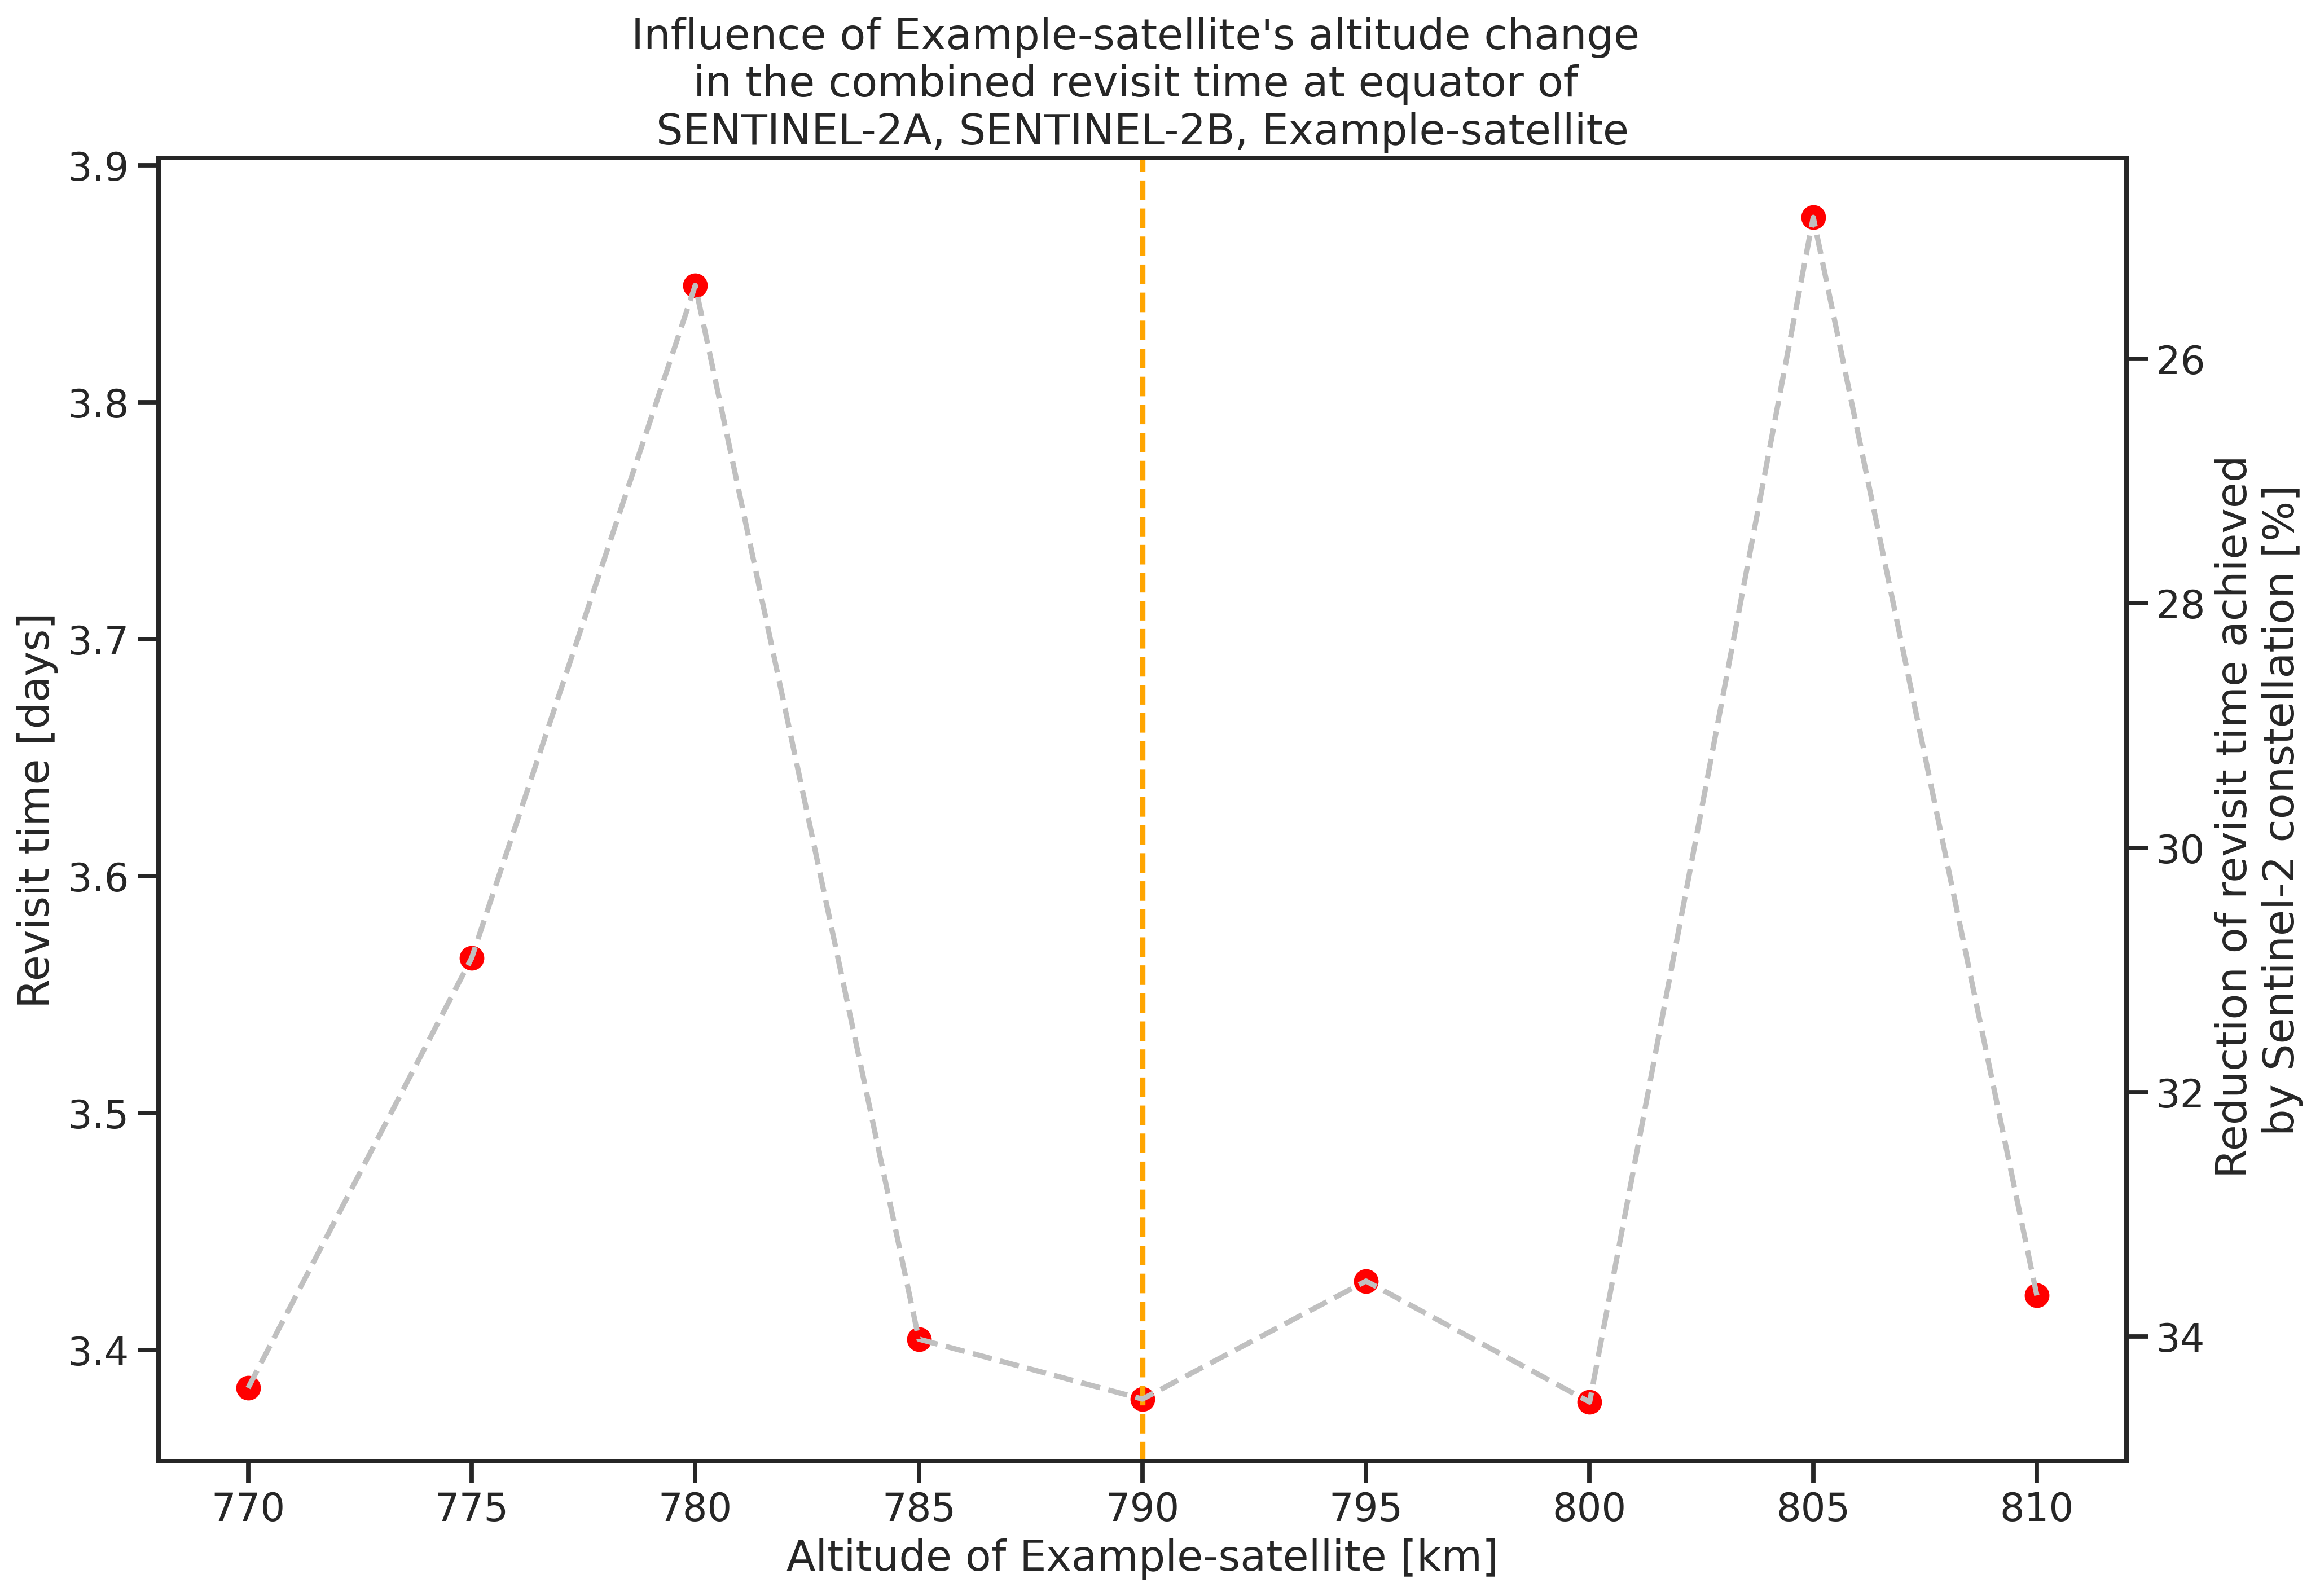
\includegraphics[width=0.9\textwidth]{Images/revisit_time_ofdoubleaxisaltitude_SENTINEL-2A_SENTINEL-2B_Example-satellite_330deg.png}
\caption{Influence of the new satellite's altitude change in the combined revisit time at equator of the Sentinel-2 constellation and the Example-satellite. The yellow line indicates the altitude of the satellites of the Sentinel-2 constellation. \underline{The mean anomaly of the Example satellite is 330 degrees.}}
\label{revisit_time_ofdoubleaxisaltitude_SENTINEL-2A_SENTINEL-2B_Example-satellite_330deg}
\end{figure}

% Code: "main_code_db_aggregated_altitude.py"
% The range of altitudes that I used for the experiment with Sentinel-2: 770-810km and omega= 83 deg.
% The range of altitudes that I used for the experiment with Flocks: 465-505km.

The constellation of the Flock-3P satellites was also used for implementing the above mentioned experiment. Firstly, an Example satellite with similar orbital characteristics to the mean characteristics of the 37 Flock-3P satellites was used to calculate the overall revisit time. Since this group of satellites is nicely distributed in the orbital plane, the experiment that is presented, pertains to the different revisit times that are achieved due to the new satellite's altitude change. These results are depicted in Figure \ref{revisit_time_ofdoubleaxisaltitude_Flocks}, in which the mean altitude of 37 Flock-3P satellites is also indicated with the yellow line.


\begin{figure}
\centering
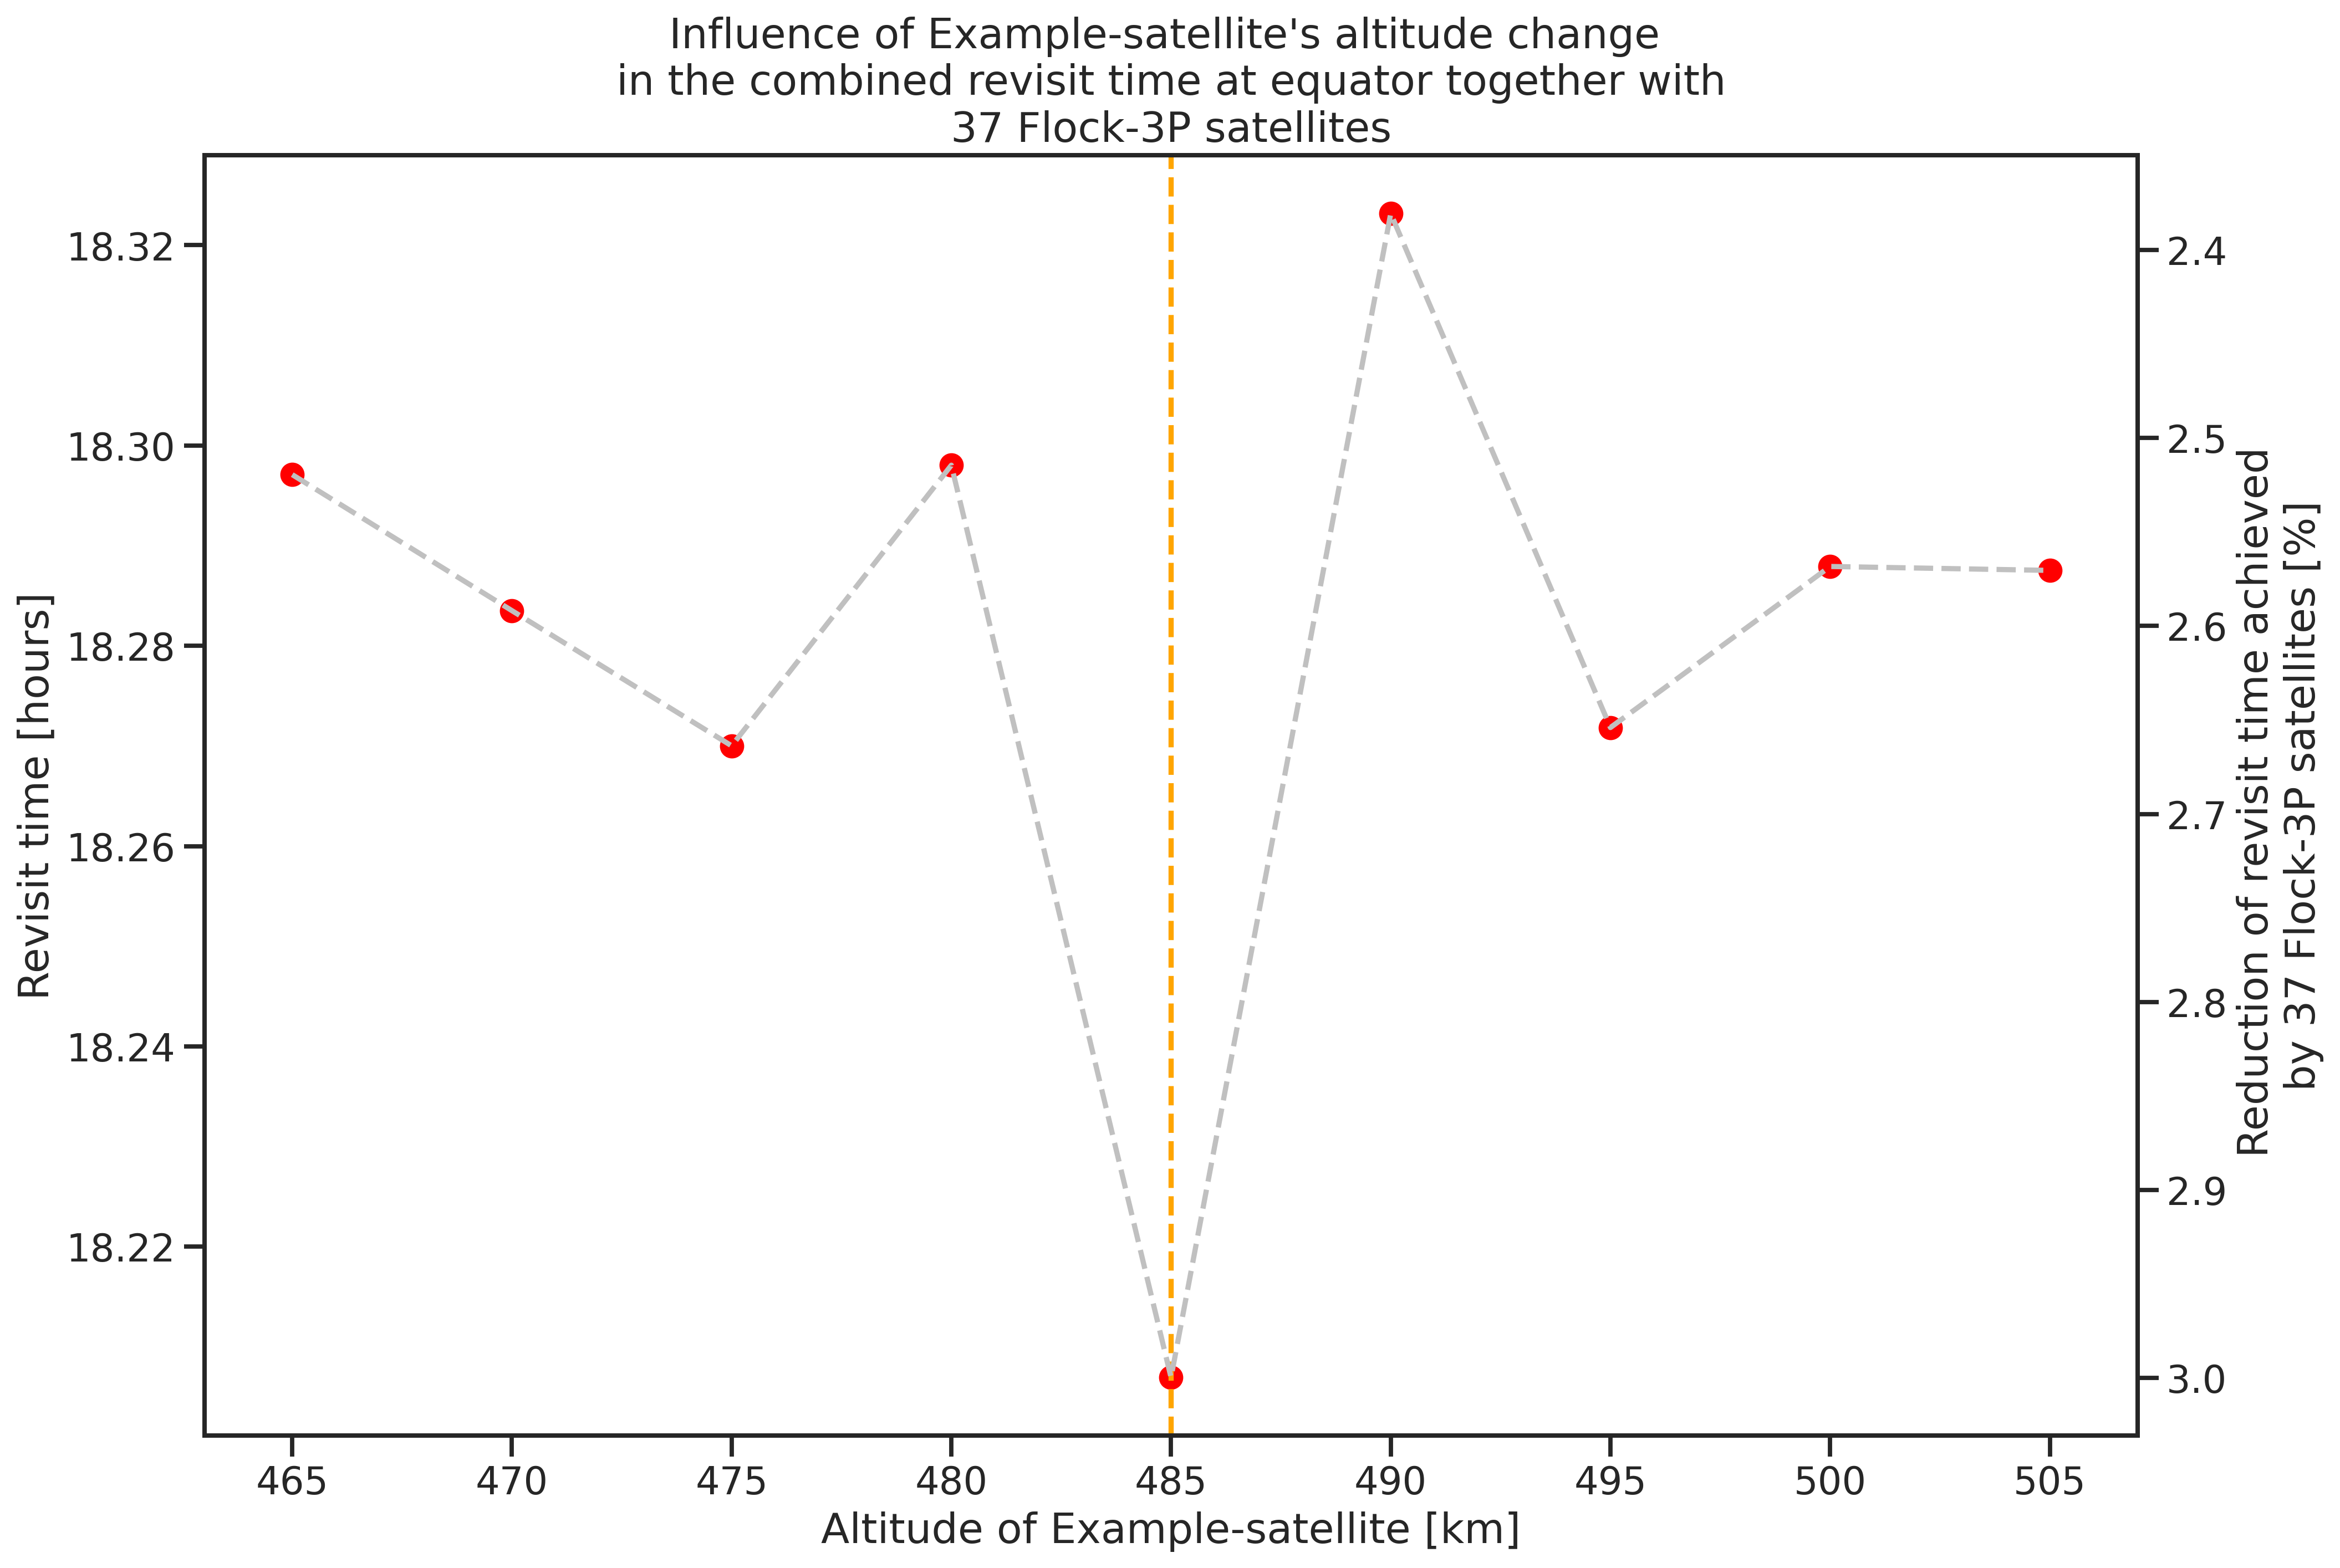
\includegraphics[width=0.9\textwidth]{Images/revisit_time_ofdoubleaxisaltitude_Flocks.png}
\caption{Influence of Example-satellite's altitude change in the combined revisit time at equator together with 37 Flock-3P satellites. The yellow line indicates the mean altitude of the satellites of the 37 Flock-3P satellites.}
\label{revisit_time_ofdoubleaxisaltitude_Flocks}
\end{figure}

\bigskip
\section{Investigation of revisit time of the entire Flock constellation}
\bigskip

The existence of proliferated constellations in the EO field has already been mentioned in table \ref{table:EO} and further information can also be found in table \ref{table:1} regarding the orbiting and operational satellites as of December 2020. However, the announcements of new launches, which will be part of already proliferated constellations, promise that the new larger fleet of satellites manages to improve the revisit time in all the part of the globe. One example company, which actualized a similar announcement recently is \textit{Planet}, promising that its constellations can revisit any part of the world seven to 12 times per day or else to revisit any place every two to four hours \footnote{\label{Flock_source}\textit{Available at: https://spacenews.com/planet-explore-2020/ (Accessed November 20, 2020)}}.

For this reason, an experiment, which can serve as a test of the revisit time of the satellite was performed. In this case, the entire Flock constellation was part of it namely 155 satellites, which are operational and in orbit as of December 2020. The average revisit time per longitude cell along the equator for this constellation can be found in Figure \ref{revisit_time_hours_of_155_Flocks}. As it can be seen, the average revisit time at equator for the constellation is almost 4 hours, which means that all the other places that have a non-zero latitude will have nearly the same or even more frequent revisit time, since the entire constellation is in near-polar orbits. 

\begin{figure}[!htb]
\centering
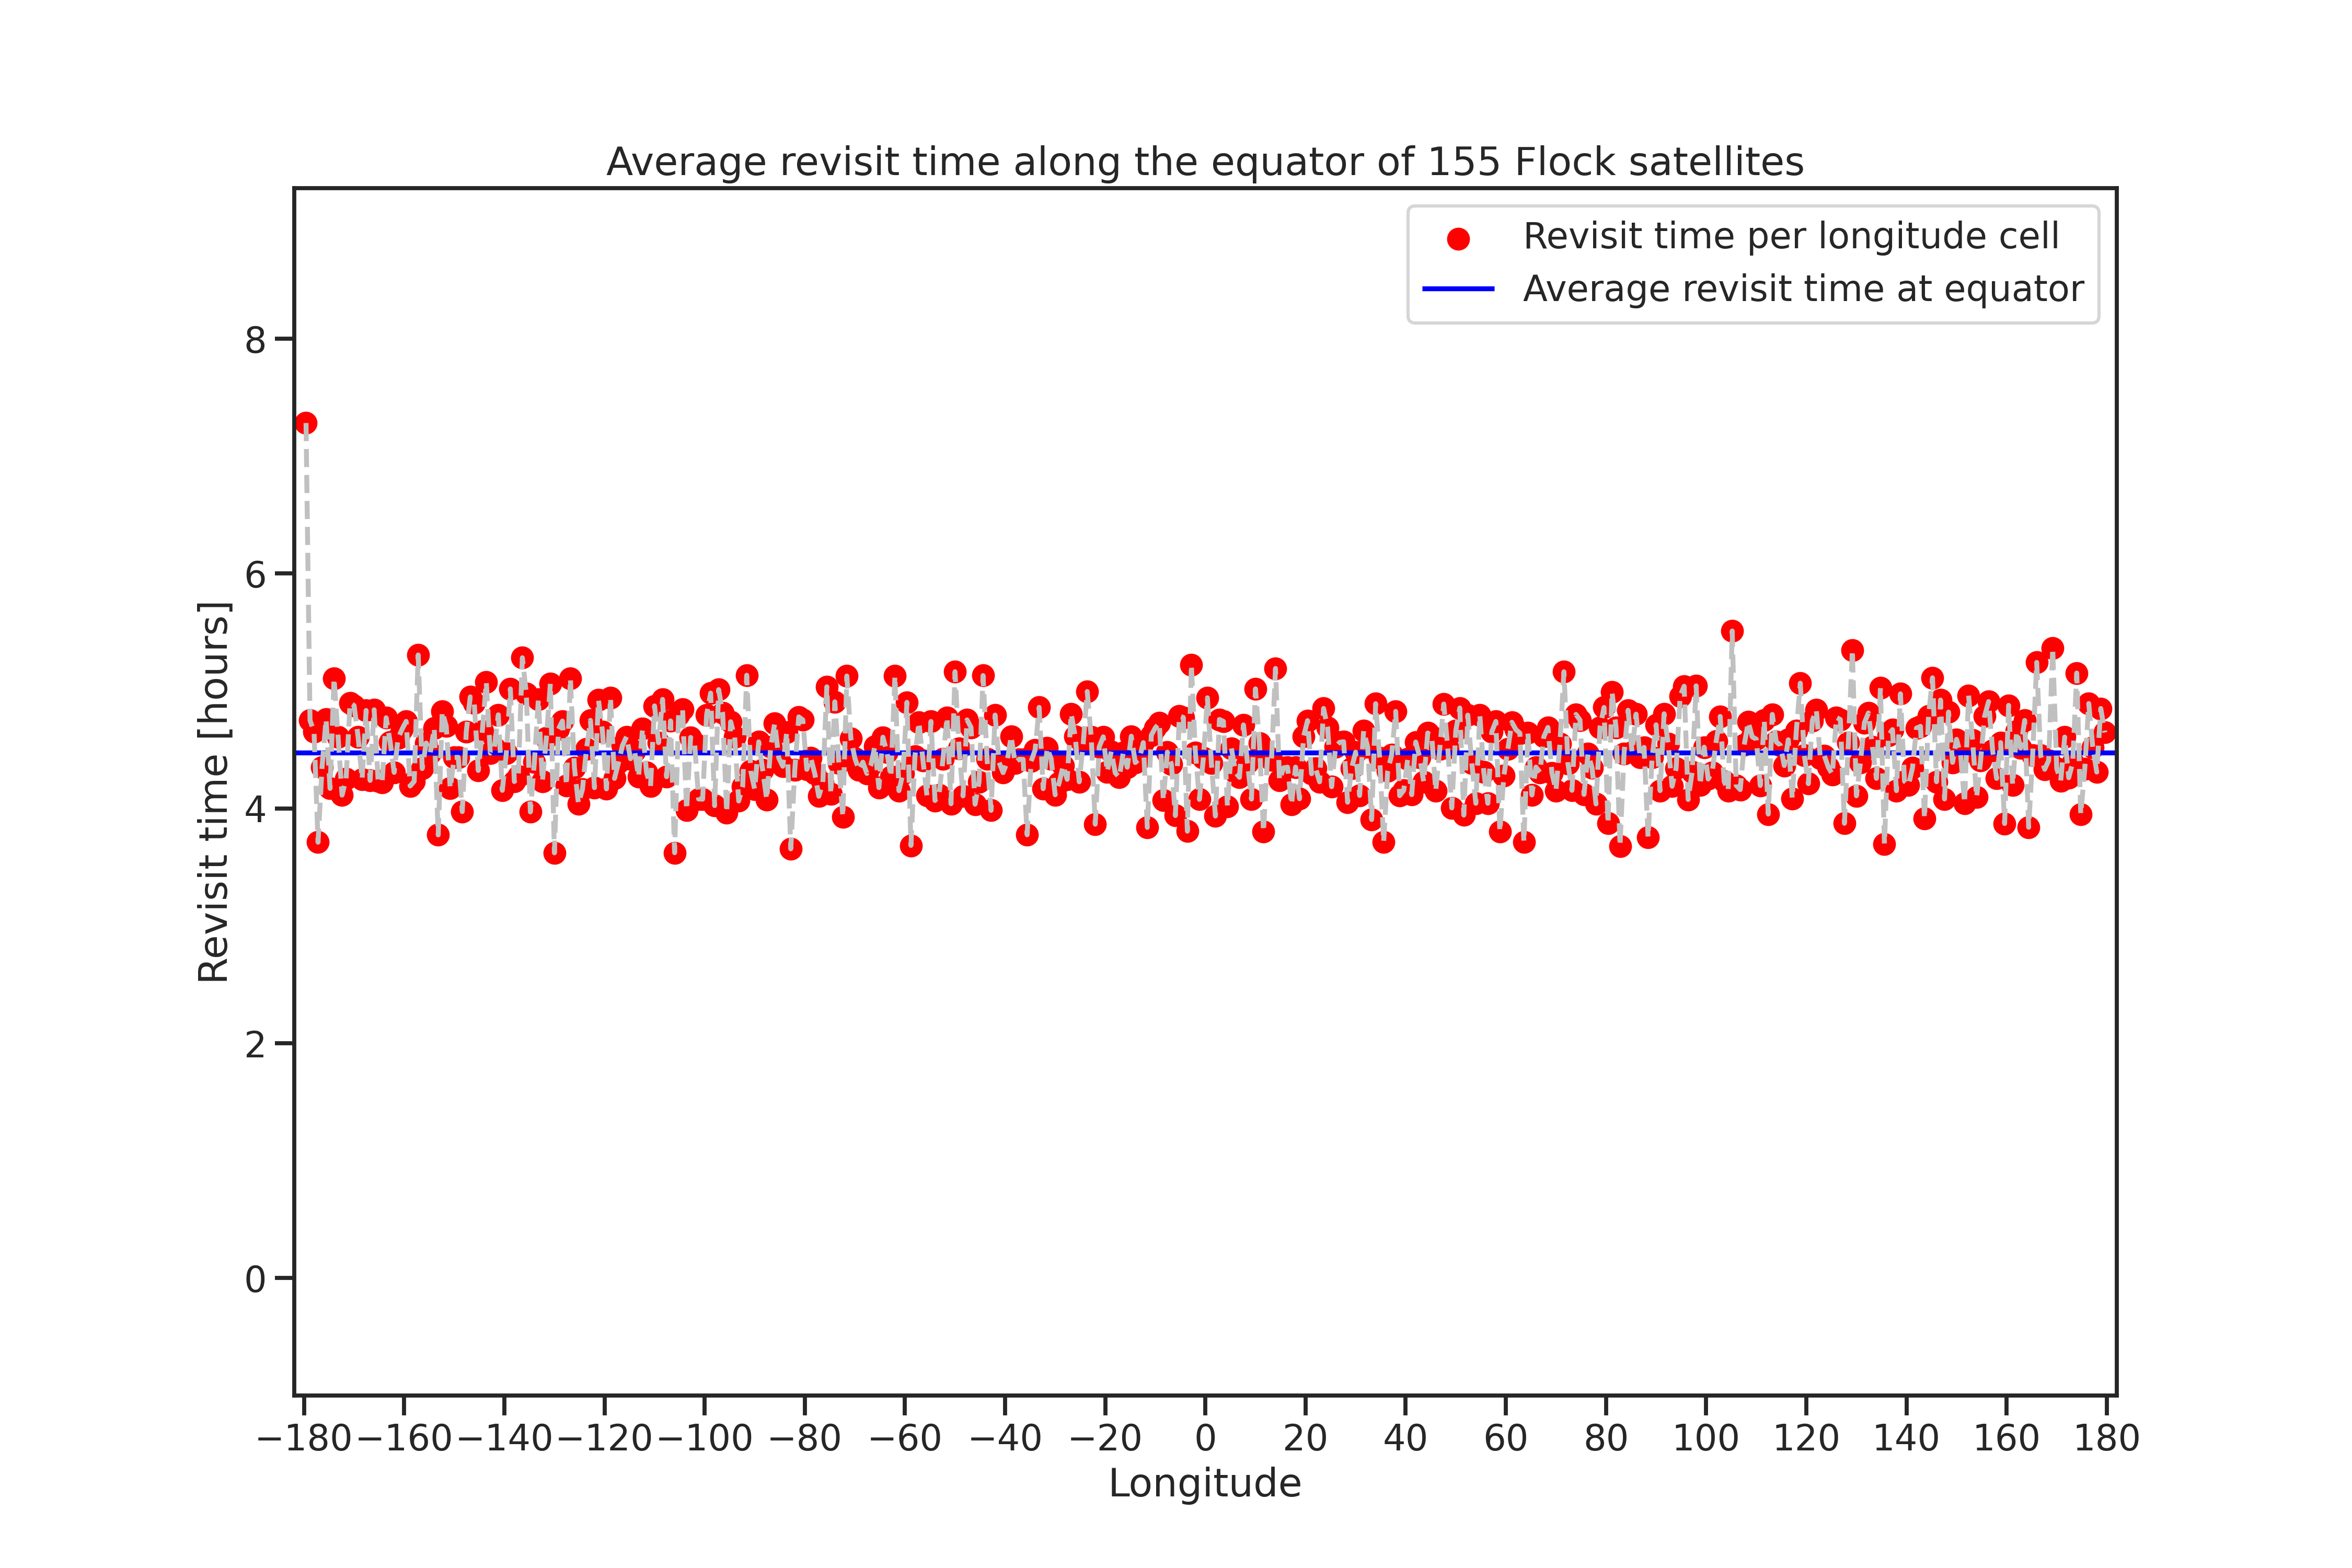
\includegraphics[width=0.9\textwidth]{Images/revisit_time_hours_of_155_Flocks.png}
\caption{Average revisit time along the equator of the entire Flock constellation - 155 satellites.}
\label{revisit_time_hours_of_155_Flocks}
\end{figure}

% Code: main_code_db_aggregated.py. I ran for all the Flocks, which are the presented all the presented id= 8-13 (and id=13!), 35-75, 77, 79-83, 86, 87, 96-142, 145-149, 151-160, 163-167, 170,171, 251-254, 256, 258-265
% BE CAREFUL!!! DONT PUT satellite_name_list in the title, or the name of the file!!!!
% Synolika, trexw gia ~ 255 Flock satellites (etsi lew kai ston pinaka sto Appendix and ston pinaka sto Chapter 1)



%\bigskip
%\section{Investigation of correlation between revisit time \& altitude}
%\bigskip
%
%\begin{figure}[!htb]
%\centering
%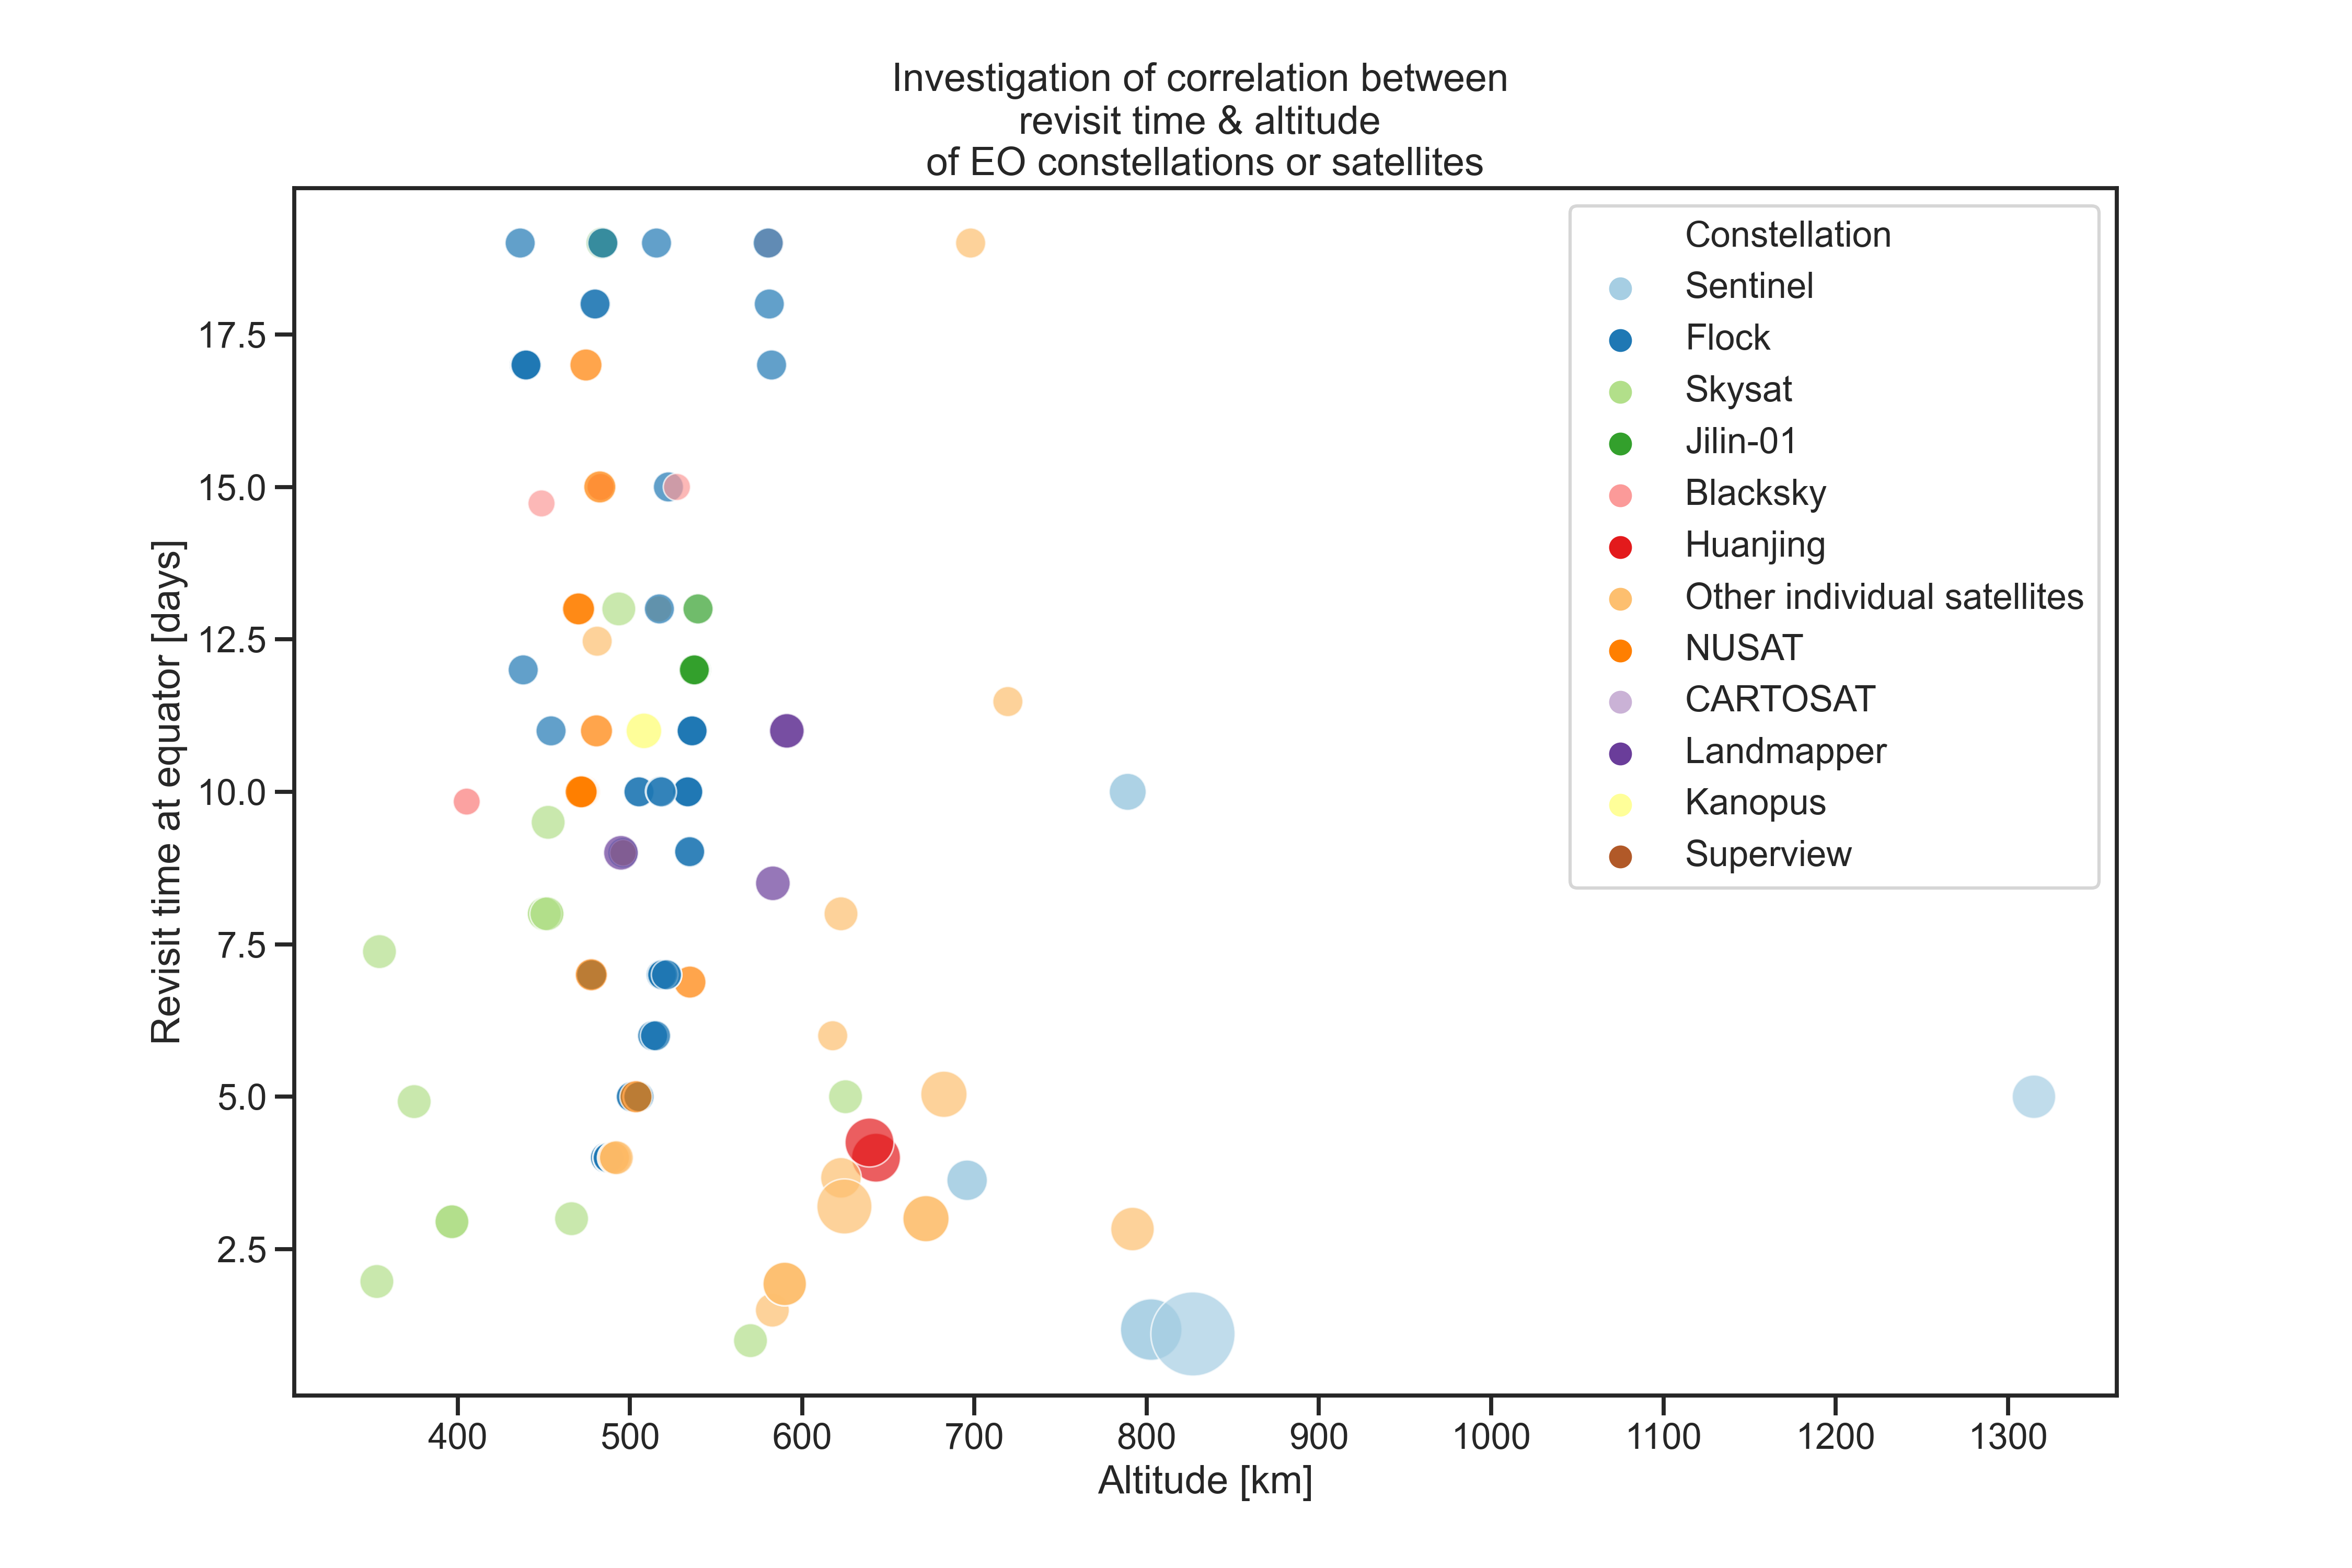
\includegraphics[width=0.9\textwidth]{Images/revisit_time_vs_altitude.png}
%\caption{Investigation of correlation between revisit time \& altitude} % Write caption smaller to wider swath width 
%\label{revisit_time_vs_altitude}
%\end{figure}
%
%% Code: revisit_altitude_plot.py